\documentclass[preprint]{elsarticle}

\usepackage{amssymb, latexsym, amsthm, amsmath,lineno,epsfig,mathtools,hyperref,todonotes,booktabs,cite}
\usepackage[singlelinecheck=false]{caption}
\modulolinenumbers[5]

\journal{Theoretical Population Biology}

%%%%%%%%%%%%%%%%%%%%%%%
%% Elsevier bibliography styles
%%%%%%%%%%%%%%%%%%%%%%%
%% To change the style, put a % in front of the second line of the current style and
%% remove the % from the second line of the style you would like to use.
%%%%%%%%%%%%%%%%%%%%%%%

%% Numbered

%\bibliographystyle{model1-num-names}

%% Numbered without titles
%\bibliographystyle{model1a-num-names}

%% Harvard
%\bibliographystyle{model2-names.bst}\biboptions{authoryear}

%% Vancouver numbered
%\usepackage{numcompress}\bibliographystyle{model3-num-names}

%% Vancouver name/year
%\usepackage{numcompress}\bibliographystyle{model4-names}\biboptions{authoryear}

%% APA style
%\bibliographystyle{model5-names}\biboptions{authoryear}

%% AMA style

%\usepackage{numcompress}\bibliographystyle{model6-num-names}

%% `Elsevier LaTeX' style
\bibliographystyle{natbibgen}
%%%%%%%%%%%%%%%%%%%%%%%

\renewcommand{\baselinestretch}{1}
\newcommand{\gdw}{\Leftrightarrow}
\newcommand{\br}{\allowdisplaybreaks}
\newcommand{\N}{\mathbb{N}}
\newcommand{\RR}{\mathbb{R}}
\newcommand{\ZZ}{\mathbb{Z}}
\newcommand{\eps}{\varepsilon}
\newcommand{\tx}{\textnormal}
\newcommand{\maxi}{\vee}
\newcommand{\mini}{\wedge}
%\newcommand{\ii}{\parallel}
\newcommand{\fett}{\textbf}
\newcommand{\T}{\textstyle}
\newcommand{\bs}[1]{\ensuremath{\boldsymbol{#1}}}

%\renewcommand{\floatpagefraction}{.8}
\newcommand\Var{\operatorname{Var}}
\newcommand\Cov{\operatorname{Cov}}
\newcommand\E{\operatorname{E}}
\newcommand\e{\operatorname{e}}
\newcommand\dbeta{\operatorname{beta}}
\newcommand\J{\operatorname{J}}
\newcommand\abs[1]{{\lvert\,#1\,\rvert}}
\newcommand\given{{\,|\,}}
\newcommand\diag[1]{{\operatorname{diag}\left(#1\right)}}
\newcommand\trps{{^{\operatorname{T}}}}
\newcommand{\norm}[1]{\left\lVert#1\right\rVert}
\newcommand\etal{{\it et~al.}}
\newcommand\eg{{\it e.g.,}}
\newcommand\cf{{\it c.f.,}}
\newcommand\ie{{\it i.e.,}}
\newcommand\bzw{{\it bzw\.}}
\newcommand\etc{{\it etc}}
\newcommand\dgr{{$^o$}}

% Dom: I decided to use X_t for time dependence instead of x(t) because it is better readable.  However, it could be redefined here, if you do not agree!
\newcommand\x[1]{\ensuremath{X_{#1}}}
% Same for y.
\newcommand\y{\ensuremath{Y}}
% Use capital or lower case letter for the time at -s?
\newcommand\s{\ensuremath{s}}
% Definitions of f, b and the one vectors.
\newcommand\fv[1]{\ensuremath{\mathbf{f}_{#1}}}
\newcommand\bv[1]{\ensuremath{\mathbf{b}_{#1}}}
\newcommand\gv[1]{\ensuremath{\mathbf{g}_{#1}}}
\newcommand\oneC{\ensuremath{\mathbf{1}'}}
\newcommand\oneR{\ensuremath{\mathbf{1}}}

\begin{document}

\begin{frontmatter}

\title{Inference in Population Genetics Using Forward and Backward, Discrete and Continuous Time Processes}

\author[address1,address2]{Juraj Bergman}
\ead{juraj.bergman@vetmeduni.ac.at}
\author[address1,address2]{Dominik Schrempf}
\ead{dominik.schrempf@vetmeduni.ac.at}
\author[address1]{Carolin Kosiol}
\ead{carolin.kosiol@vetmeduni.ac.at}
\author[address3]{Claus Vogl\corref{correspondingauthor}}
\cortext[correspondingauthor]{Corresponding author}
\ead{claus.vogl@vetmeduni.ac.at}

\address[address1]{Institut f\"ur Populationsgenetik, Vetmeduni Vienna, Veterin\"arplatz 1, A-1210 Wien, Austria}
\address[address2]{Vienna Graduate School of Population Genetics, A-1210 Wien, Austria}
\address[address3]{Institut f\"ur Tierzucht und Genetik, Vetmeduni Vienna, Veterin\"arplatz 1, A-1210 Wien, Austria}

\begin{abstract}
The Wright-Fisher and Moran models are Markov processes, where discrete population allele frequencies are iterated forward in time by multiplication with a transition matrix, modeling population genetic forces (\eg\ mutation, selection, and drift). For large population sizes, iteration can be replaced by continuous diffusion. Data are typically aligned sequences of a sample of individuals from one or more populations from the present that can be represented as site frequency spectra (SFS) of a single population or joint site frequency spectra (jSFS) of many populations, respectively. The task is to infer population genetic parameters or the population history from the data. With forward processes, \ie\ the Wright-Fisher, the Moran, or the forward diffusion models, population allele frequency distributions in and out of equilibrium may be obtained. These can be combined with the likelihoods of an SFS to obtain joint distributions of sample and population allele frequencies. By integrating out population allele frequencies, population genetic parameters may be obtained from the marginal likelihoods. Backward processes consist of, in the discrete case, iteration of the transpose of the transition matrix or, in the continuous case, of the backward diffusion equation. We make use of the the forward and backward processes, as in the forward-backward algorithm of hidden Markov models, to efficiently calculate the probability distribution of population allele frequencies at all times in the past. Additionally, marginal likelihoods of samples from multiple populations that split in the past, \ie\ of a jSFS, may be obtained.
\end{abstract}
\begin{keyword}
bi-allelic mutation-drift models \sep Markov chain \sep time reversal \sep forward and backward diffusion \sep conditional allele frequency distribution \sep inference.
\end{keyword}

\end{frontmatter}

\linenumbers

\listoftodos

\section{Introduction}

Most basic population genetic models, \eg\ the Wright-Fisher and the Moran models as well as the forward and backward diffusion models \citep[reviewed in][]{Ewen04}, were introduced before DNA sequence data became available. Thus, emphasis was on demonstrating processes over time and on qualitatively explaining observations, rather than on quantitative inference of population genetic parameters given molecular data. On the other hand, coalescent theory \citep{King82} was used both for demonstration of processes as well as for inference given a population sample \citep{Hein05,Wake09}. With coalescence, the history of a particular sample is reconstructed, however the aim in population genetics is most often the inference of the evolutionary trajectory of the whole population.

In regions of relatively high recombination rates compared to mutation rates, sites may be assumed to evolve independently. Usually, mutation rates are low such that most sites in, \eg\ \textit{Drosophila} or mammal population samples are monomorphic (fixed), while only two bases segregate at polymorphic sites. Therefore, most genomic sites are bi-allelic with respect to their nucleotide composition or when compared to an ancestral state. %Population data are usually represented as a site frequency spectrum (SFS) for a single population or a joint site frequency spectrum (jSFS), for two populations that split some time in the past.

Typically, the data $Y$ are from the present time and consist of an alignment of $M$ sequences (randomly drawn from a population) across $L$ sites. Such a dataset can be represented as an SFS whose likelihood can be calculated given the present population allele frequency $X_0$ and a probability model describing the sampling process. The distribution of $X_0$ is in turn given by a population genetic model parametrized by, \eg\ the scaled mutation rate $\theta=N\mu$, the mutation bias $\alpha$, or the selection strength $\gamma=Ns$ \citep[as defined in][]{Vogl15}. Integrating over all values of $X_0$, the marginal likelihood $\Pr(Y\given \alpha,\theta,\gamma)$ may be obtained and maximum likelihood inference of population genetic parameters is possible under the assumption of equilibrium \citep{Vogl14b,Vogl15}. This strategy may also be viewed as the empirical Bayes method \citep[\eg][]{Carl00}. 

Maximum likelihood inference is more complicated with data from two or more populations that split some time in the past, represented by a jSFS. Models iterating forward in time such as the Wright-Fisher, Moran or continuous diffusion models, have rarely been used for this task. An exception is the forward iteration of a Moran model in phylogenetic inference \citep{Schrempf2016}. In this case, summation over all $N+1$ ancestral states is necessary at each node, \ie\ at each binary split into two populations. Such summation becomes difficult with large $N$. Therefore, mutation rates are scaled such that $N$ can be taken small. Note that sample sizes $M$ can be large for sequence data from pooled individuals or from many populations and information is inevitably lost if $M>N$. Therefore, such data are  difficult to analyze accurately with forward methods. %Note that diagonalization of the transition matrix is necessary for numerical efficiency. %CV: I would want to leave Zhao14 in the intro, lest we only introducing our own research!
%Moreover,
\citet{Zhao14} provide a forward algorithm based on the Wright-Fisher model, where probabilities of intermediate states are calculated conditional on the starting and end states. This allows for simulation of trajectories. 

Backward processes can be used to calculate the likelihood of the data $Y$ conditional on the population allele frequency $X_t$  at earlier times ($t<0$). %allow pushing the conditioning on the population allele frequency backward in time, \ie\ they allow calculation of the likelihood $\Pr(Y\given X_t, \dots)$ with $t<0$.
In the discrete case, the process consists of iterating the transpose of the forward transition matrix; in the continuous case, a solution to the backwards diffusion equation is needed.
%They consist of, in the discrete case, iteration of the transpose of the forward transition matrix; in the continuous case, of the backward diffusion equation.
Combining the forward and backward processes in the forward-backward algorithm of hidden Markov models (HMM) \citep{Rabi86}, the probability distribution of population allele frequencies conditional on data $\Pr(X_t\given Y,\dots)$ can be inferred at time $t$ in the past and the distribution of trajectories may be simulated. This may be an aim in itself \citep{Zhao14}. Additionally, it is  possible to calculate the marginal likelihoods of samples from multiple splitting populations, \ie\ from a jSFS, by integrating out the population allele frequencies.

In this article, we use forward and backward processes to conveniently calculate the probability distirbution of $X_t$ forward and backward in time conditional on the SFS or the jSFS from the present. %In discrete time, this corresponds to a variant of the forward-backward algorithm \citep{Rabi86}. The method can also be used to calculate likelihoods of jSFS. 
Furthermore, we introduce bi-allelic population genetic models, with mutations occurring only at fixed sites that are variants of the infinite site or Poisson-random-fields models \citep{Kimu69,Sawy92}. The Markov chains of the models under consideration have no absorbing states and therefore have stationary distributions. However, we do not always assume time-reversibility.

For the discrete models, matrix multiplication is necessary to iterate the distribution of population allele frequencies forward and backward in time. The size of the transition matrix depends on the population size $N$ and multiplication can become cumbersome if $N$ is large. However, the size of the matrix can be reduced by appropriate rescaling of population genetic parameters.

In the limit $N\to\infty$, the solution to the corresponding Kolmogorov forward and backward diffusion equations is obtained. With mutation and drift only, orthogonal polynomials provide a flexible and fast method to solve the diffusion equations and calculate marginal likelihoods for inference in population genetics.

\section{Time-homogeneous discrete Markov chains}

In this section we apply the forward-backward algorithm to discrete population genetic models for inference given an SFS or jSFS. To this purpose, we rephrase iteration using discrete population genetic models (Wright-Fisher or Moran) in the terminology of the forward-backward algorithm. We mainly use matrix notation to emphasize the similarities between discrete iteration and continuous models in Sections~\ref{forwBackDiff} and ~\ref{section:diffDer}. Many subsections review standard theory, but are included for completeness and clarity. 

\subsection{Assumptions}\label{section:assumptions}
\begin{enumerate}[(i)]
\item Assume a population of large (effective) size $N$ and some bi-allelic mutation model. The time-dependent frequency of allele zero in the population is denoted $\x{t}$ ($0 \le \x{t} \le N$) and is assumed to evolve as a discrete, time-homogeneous Markov chain with a transition probability matrix $\mathbf{T}$, where $(T_{ij})_{i,j \in \{0, \ldots, N\}} = \Pr(\x{t+1}=j \given \x{t}=i)$. $\mathbf{T}$ is an irreducible, aperiodic, right stochastic matrix.
\item At a (possibly unknown) time $t=\s$ ($\s<0$) in the past, a distribution of population allelic proportions is given by $\bs{\rho}$ with entries $(\rho_{i})_{i \in \{0, \ldots, N\}} = \Pr(\x{\s}=i)$.  In particular, $\bs{\rho}$ may be the stationary distribution of the forward process $\bs{\pi}=(\pi_i)_{i \in \{0, \ldots, N\}}$ or may correspond to a joint distribution of some other data and the equilibrium allele frequency distribution. 
\item The population evolves until the present time $t=0$, when a sample of size $M$ is drawn.  We denote the sampled frequency of allele zero as $\y$ ($0 \le \y \le M$). The likelihood of observing $\y$ is given by $\Pr(\y \given M, \x{0})$ (we may leave away the dependency on $M$ in the following) and will be defined according to the application.
\end{enumerate}

For two populations, assumptions (ii) and (iii) are modified:
\begin{enumerate}[(i)]
\setcounter{enumi}{1}
\item At a (possibly unknown) time $t=\s$ ($\s<0$) in the past,  $\x{\s}$ is drawn from a distribution of population allelic proportions $\bs{\rho}$. The population separates immediately into two populations with the same initial allele frequency $\x{\s}$. 
\item The two populations evolve independently until the present time $t=0$, when samples of sizes $M_1$ and $M_2$ are drawn from each population.
\end{enumerate}

For discrete models, iteration is more efficient if the population size $N$ is small. $N$ can be decreased by increasing the mutation rate $\mu$ such that $\theta=N \mu$ remains constant. For moderate $N$, the error introduced by scaling is small and converges to $0$ in the diffusion limit $N \to \infty$. Therefore, $N$ is usually set according to numerical convenience. %Furthermore, adjusting $\mu$ does not change the state space and is thus more convenient than adjusting $N$.

%For the discrete models, note that $\theta$ corresponds to the mutation rate scaled with the effective population size. A small population size $N$ leads to more efficient iteration and for moderate $N$ changing the mutation rate is almost indistinguishable from changing the population size (and becomes identical in the diffusion limit of $N\to\infty$). Therefore, $N$ is usually set for numerical convenience and the mutation rate $\mu$ is adjusted to achieve realistic $\theta$, such that $\mu=\theta/N$. Furthermore, adjusting $\mu$ does not change the state space and is thus more convenient than adjusting $N$.

\subsection{Forward in time}

Often, our data are from the present and we want to condition on the configuration of allele frequencies at earlier times.  We introduce the row vector $\fv{t}$ with entries $(\fv{t})_{i} = \Pr(X_{t} = i)$ and set $\fv{\s} = \bs{\rho}$, \ie\ to the vector of initial probabilities of states. We can calculate the vector of probabilities of states recursively 
\begin{equation}
\fv{t+1} = \fv{t}\mathbf{T} \quad (\s \le t \le -1).
\end{equation}
This corresponds to the recursion in the forward algorithm in the theory of Hidden Markov models (HMM)~\citep[\eg][]{Vogl10}. Let $\oneC$ be a column vector of ones ($'$ depicts matrix transposition) and $\mathbf{D}$ a diagonal matrix with the conditional likelihoods on the main diagonal, \ie\ $(\mathbf{D})_{ii}=\Pr(\y \given \x{0}=i)$. The marginal likelihood then is
\begin{equation}
\Pr(\y \given \bs{\rho}) = \fv{\s}\mathbf{T}^{|\s|}\mathbf{D}\oneC.
\end{equation}

\subsection{Backward in time}\label{section:backward}

Using a strategy as with the backward algorithm in the theory of HMM, set $\bv{0}'=\mathbf{D}\oneC$. Backward in time, the recursion is
\begin{equation}
\begin{split}
\bv{t}' = \mathbf{T} \bv{t+1}' \quad (\s \le t \le -1),
\end{split}
\end{equation}
which can also be written as
\begin{equation}\label{eq:backwards_discrete}
\begin{split}
\Pr(\y \given \x{t}=i) = \sum_j \Pr(\x{t+1}=j \given \x{t}=i) \Pr(\y \given \x{t+1}=j).
%&=\sum_j q_{ij} \Pr(\y \given \x{t+1}=j).
\end{split}
\end{equation}
From the definition of $\bv{t}$, it follows that we condition on $\x{t}$
\begin{equation}
(\bv{t})_{i} = \Pr(\y \given \x{t}=i).
\end{equation}
The recursion moves the conditioning to ever earlier times. The marginal likelihood may also be obtained with the backward algorithm,
\begin{equation}\label{eq:marg_lh}
\begin{split}
\Pr(\y \given \bs{\rho}) &= \fv{\s} \left[\mathbf{T}^{|\s|} \mathbf{D}\oneC\right]\\
                         &= \fv{\s} \bv{\s}' \\
                         &= \sum_i \rho_i \Pr(\y \given \x{\s}=i).
\end{split}
\end{equation}

\subsection{Constancy of the marginal distribution and adjointness}

The marginal likelihood (\ref{eq:marg_lh}) is constant over time $t$ 
\begin{equation}
\Pr(\y \given \bs{\rho}) = \fv{t}\bv{t}' =\sum_i \Pr(\x{t}=i \given \bs{\rho}) \Pr(\y \given \x{t}=i) = \norm{ \fv{t}, \bv{t} },
\end{equation}
where $\norm{ \cdot , \cdot }$ denotes an inner product.  It follows that forward and backward transition matrices, \ie\ $\mathbf{T}$ and its transpose $\mathbf{T}'$, are adjoint since
\begin{equation}\label{eq:adjoint_discrete}
\begin{split}
\Pr(\y \given \bs{\rho})              &= \Pr(\y \given \bs{\rho}) \\
(\fv{t}\mathbf{T})\bv{t+1}' &= \fv{t} (\mathbf{T}\bv{t+1}') \\
\norm{ \fv{t}\mathbf{T},\bv{t+1} }  &= \norm{\fv{t},\bv{t+1}\mathbf{T}' }.
\end{split}
\end{equation}
Like a zipper, this adjoint relationship allows movement forward and backward in time.

\subsection{Joint and conditional distribution}

The probability of $\x{t}$ and $\y$ conditional on the starting distribution $\bs{\rho}$ is \begin{equation}\label{eq:joint_xy_discr}
\Pr(\x{t}=i,\y \given \bs{\rho}) = (\fv{t})_i (\bv{t})_i\,.
\end{equation}
Furthermore, the probability of $\x{t}$ conditional on the data and the starting distribution is
\begin{equation}\label{eq:cond_x|y_discr}
\Pr(\x{t}=i \given \y,\bs{\rho}) = \frac{(\fv{t})_i (\bv{t})_i}{\fv{t}\bv{t}'}\,.
\end{equation}
This allows calculation of the distribution of population allele frequencies conditional on the data at any time. 

\subsection{Sampling from conditional trajectories}

It is possible to simulate trajectories given the initial distribution $\bs{\rho}$ at time $\s$ and the likelihood at time $t=0$. Note that \citet{Zhao14} provide a similar algorithm based on the Wright-Fisher model to simulate trajectories of population allelic proportions conditional on the starting and end states. In contrast, we start with a sample at time $t=\s$ from the conditional probabilities (\ref{eq:cond_x|y_discr}). Given the state at time $t-1$ the probability of the state at time $t$ is
\begin{equation}
    \Pr(\x{t}=j\given \x{t-1}=i,\y)=\frac{(\mathbf{T})_{ij}(\mathbf{b}_{t})_j}{(\mathbf{b}_{t-1})_i}\,,
\end{equation}
which can be used to obtain a sample trajectory. For $t>s$ the formula does not contain $\bs{\rho}$ since it is a Markov process.

\subsection{Left and right eigenvectors, stationary distribution}

Let $\bs{\pi} = (\pi_i)_{i \in \{0,\ldots,N\}}$ be the stationary distribution of $\mathbf{T}$, if it exists. $\bs{\pi}$ is the left eigenvector associated with the largest eigenvalue one~\citep[][p. 87]{Ewen04}
\begin{equation}\label{eq:stationary}
\bs{\pi}=\bs{\pi}\mathbf{T}.
\end{equation}
All entries of $\bs{\pi}$ are greater than zero because the transition matrix was assumed to be irreducible and $\sum \pi_i = 1$. Thus the entries of $\bs{\pi}$ can be interpreted as probabilities. Since the rows of $\mathbf{T}$ sum to one, it is obvious that a column vector of all ones $\oneC$ is the right eigenvector associated with the unit eigenvalue. In our context, this means that iterating forward in time will converge to a vector proportional to $\bs{\pi}$ and iterating backward in time to a vector proportional to $\oneC$. Thus, every state is equally likely when  $s\to-\infty$. % CV: The backward algorithm does not conserve the total probability mass. Hence, going backward is only proportional to $\oneR$.

\subsection{Reversibility}

Define the diagonal matrix $\mathbf{\Pi}$ with the entries $\pi_i$ on the main diagonal. Since irreducible Markov chains with finite state space have stationary distributions with only strictly positive entries, $\mathbf{\Pi}$ is invertible with $\mathbf{\Pi}^{-1}$ being a diagonal matrix with entries $1/\pi_i$.  Set
\begin{equation}\label{eq:reverse_transition}
\begin{split}
\mathbf{T}^{*}=\mathbf{\Pi}\mathbf{T}\mathbf{\Pi}^{-1}\,.
\end{split}
\end{equation}
The Markov chain is reversible, if $\mathbf{T}^{*}=\mathbf{T}'$, because then
\begin{equation}\label{eq:detailed_balance}
\begin{split}
  \mathbf{T}' &= \mathbf{T}^{*} \\
             &= \mathbf{\Pi}\mathbf{T}\mathbf{\Pi}^{-1}, \text{ or} \\
  \mathbf{T}'\mathbf{\Pi} &= \mathbf{\Pi T},
\end{split}
\end{equation}
which corresponds to detailed balance.
%This condition corresponds to a balanced flow between any pair of states, \ie\ the conditions of detailed balance
% \begin{align}
% \pi_i \Pr(\x{t+1}=j \given \x{t}=i)
%                               &=  \pi_j \Pr(\x{t+1}=i \given \x{t}=j).
% \end{align}

We can separate $\fv{t}$ into a product of a time dependent row vector $\gv{t}$ and the stationary distribution matrix $\mathbf{\Pi}$
\begin{equation}\label{decomp}
\fv{t}=\gv{t}\mathbf{\Pi}.
\end{equation}
Under reversibility, we have forward in time
\begin{equation}
\begin{split}
\gv{t+1}\mathbf{\Pi} &=\gv{t}\mathbf{\Pi}\mathbf{T}\\
\gv{t+1}             &=\gv{t}\mathbf{\Pi}\mathbf{T}\mathbf{\Pi}^{-1}\\
\gv{t+1}             &=\gv{t}\mathbf{T}'\,.
\end{split}
\end{equation}
Thus the ``backward'' transition matrix $\mathbf{T}'$ may be used forward and backward in time. We may interpret $\gv{t}$
% with entries:
% TODO CV and DS:
% DS: Ich glaube, das ist nicht richtig.  Wo kommt Y her?
% CV: ich glaube:
% $(\gv{t})_i=\Pr(\y_{t}\given y_{s},y_{s+1},\dots,y_{t-1},\x{t}=i)$
% DS: ist Y nicht das Sample?  Macht es Sinn Y_t zu schreiben?  Ich interpretiere g_t als ein Maß für die Entfernung vom stationären Zustand.  Ich bin mir nicht sicher, ob man dieses Maß als Likelihood oder Wahrscheinlichkeit interpretieren kann. 
%CV: Red ma drueber...
as a ``projected likelihood'' that, when multiplied with the stationary distribution, gives the joint distribution $\fv{t}$. Note that with the decomposition (\ref{decomp}), the likelihood becomes
\begin{equation}
\Pr(\y \given \bs{\rho}) = \gv{t} \mathbf{\Pi} \bv{t}'.
\end{equation}
The adjoint relationship~(\ref{eq:adjoint_discrete}) can be modified analogously, to result in the self-adjoint relationship
\begin{equation}\label{eq:adjoint_discrete_2}
\begin{split}
\Pr(\y \given \bs{\rho})                              & = \Pr(\y \given \bs{\rho})                    \\
(\gv{t}\mathbf{\Pi} \mathbf{T}) \bv{t+1}'             & = \gv{t}(\mathbf{T}^{'}\mathbf{\Pi}\bv{t+1}') \\
\norm{ \gv{t}\mathbf{\Pi}\mathbf{T},\bv{t+1}}         & = 
\norm{ \gv{t},\bv{t+1}\mathbf{\Pi}\mathbf{T} }.
\end{split}
\end{equation}

\subsection{Example: Conditional probabilities under irreversible mutation}\label{section:irreversible}

As a particular realization of a discrete process consider a bi-allelic model, where alleles can be labeled either as ancestral (zero) or derived (one). Mutation rates are assumed to be small (at most one mutation is segregating per site) and limited to the boundary zero, \ie\ when a derived allele is fixed, it immediately becomes ancestral. This process is a variant of the infinite sites model \citep{Kimu69} and similar to the Poisson-random-fields model \citep{Sawy92}, but differs in that it allows for a stationary distribution. Using diffusion theory, \citet{Evan07} provide an analysis based on moments of the allelic proportions of a similar model with mutations from only one boundary, assuming changing population sizes, \ie\ not assuming equilibrium. \citet{Zivk15} extend the analysis to include selection. 

The transition matrix $\mathbf{T}$ is defined as follows. Given a time-homogeneous mutation rate $\mu$, transition probabilities at the boundary zero are
\begin{equation}\label{eq:boundary_mutation}
\begin{cases}
\Pr(\x{t+1}=0\given \x{t}=0)&=1-\mu/(1-\theta\sum_{i=1}^{N-1}1/i)\\
\Pr(\x{t+1}=1\given \x{t}=0)&=\mu/(1-\theta\sum_{i=1}^{N-1}1/i),
\end{cases}
\end{equation}
where $\theta=\mu N$. Within the polymorphic region, random drift is the only force affecting allele frequencies, such that for $1\leq i \leq N-2$
\begin{equation}
\begin{cases}
\Pr(\x{t+1}=i-1\given \x{t}=i) &=\frac1{N^2} i(N-i)\\
\Pr(\x{t+1}=i\given \x{t}=i)   &=1-\frac1{N^2} 2i(N-i)\\
\Pr(\x{t+1}=i+1\given \x{t}=i) &=\frac1{N^2} i(N-i)\,.
\end{cases}
\end{equation}
For $i=N-1$, drift may lead to fixation of the derived allele, which then becomes the ancestral allele, \ie\
\begin{equation}
\begin{cases}
\Pr(\x{t+1}=N-2\given \x{t}=N-1) &=\frac1{N^2} (N-1)\\
\Pr(\x{t+1}=N-1\given \x{t}=N-1) &=1-\frac1{N^2} 2(N-1)\\
\Pr(\x{t+1}=0\given \x{t}=N-1)   &=\frac1{N^2} (N-1)\,.
\end{cases}
\end{equation}
The state $N$ is never reached and is left out of the state space. The system is not in detailed balance, as probability mass moves from $i=N-1$ to $i=0$, but not in the reverse direction.

The stationary distribution  is 
\begin{equation}\label{eq_dist}
\bs{\pi}(i)=\begin{cases}
\Pr(\x{}=0)&=1-\theta\sum_{i=1}^{N-1}1/i\\
\Pr(\x{}=i)_{i \in \{1, \ldots, N-1\}} &=\theta/i\,,
\end{cases}
\end{equation}
as can be ascertained by substitution.

As an example of a demographic scenario (Fig.~\ref{diag}A), consider a population with a stationary allele frequency distribution \eqref{eq_dist} defined by the ancestral mutation rate $\mu_a$ at some time $s$ in the past; \ie\ $\bs{\rho} = \bs{\pi_a}$. Furthermore, assume an instantaneous expansion of the population size between generations $s$ and $s+1$. From then on, the population is out of equilibrium and evolving with a new current mutation rate $\mu_c$. At present time ($t=0$), 
we sample $M$ haplotypes from the population. Assume that the ancestral state of the sampled haplotypes can be determined without error. Thus, a polarized SFS may be constructed. For any value of $\mu_c$ and $N$, a transition matrix $\mathbf{T}$ can be calculated using the described framework. Furthermore, the matrix $\mathbf{T}^{'}$ can be used to iterate the conditioning of the allele frequency distribution backwards in time. Assume a hypergeometric distribution of $Y$, conditional on $N$, $i$, and $M$
\begin{equation}\label{X0}
\Pr(\y\given N,i,M)=\frac{\binom{i}{\y}\binom{N-i}{M-\y}}{\binom{N}{M}}\,,
\end{equation}
where $0\leq \y\leq M$ and $0\leq i\leq (N-1)$. The conditional probabilities of allelic states $\Pr(\y \given \bs{\rho})$, for any time $s\leq t\leq 0$, in a site frequency spectrum of size $M$ can then be calculated (Fig.~\ref{cProb}). %For inference given a SFS, the marginal likelihood can be maximized by searching the parameter spaces of $\mu_a$, $\mu_c$, and $t$.

\subsection{Example: Joint site frequency spectrum under reversible mutation}\label{section:discr_rev_general}
As another realization of a discrete process consider a bi-allelic mutation-drift decoupled Moran model~\citep{Baak08,Ethe09} with haploid population size $N$, mutation rate towards zero $\mu_0$ and mutation rate towards one $\mu_1$ ($\mu=\mu_0+\mu_1$).  We introduce the parameters $\alpha=\mu_1/\mu$ ($0 \leq \alpha \leq 1$) and $\beta=1-\alpha=\mu_0/\mu$ which are the mutation biases towards allele one and zero, respectively.  Let $i$ ($0\leq i\leq N$) be the frequency of allele one. Then, the tri-diagonal transition rate matrix $\mathbf{T}$ depends on $N$, $\mu$ and $\alpha$
\begin{equation}\label{eq:transition_decoupled_Moran}
\begin{cases}
\Pr(\x{t+1}=i-1\given \x{t}=i)&=\frac{i(N-i)}{N^2}+\beta\mu \frac{i}{N}\\
    \Pr(\x{t+1}=i\given \x{t}=i)&=1-\frac{2i(N-i)}{N^2}+\beta\mu \frac{i}{N} + \alpha\mu \frac{N-i}N\\
\Pr(\x{t+1}=i+1\given \x{t}=i)&=\frac{i(N-i)}{N^2}+\alpha\mu \frac{N-i}N\,.
\end{cases}
\end{equation}

The stationary distribution of $\x{}$ is a beta-binomial
\begin{equation}\label{beta_bin}
\Pr(\x{}=i\given N,\alpha,\theta)=\binom{N}{i}
\frac{\Gamma(\theta)}{\Gamma(\alpha\theta)\Gamma(\beta\theta)}
\frac{\Gamma(i+\alpha\theta)\Gamma(N-i+\beta\theta)}{\Gamma(N+\theta)}\,.
\end{equation}
The assertion can be verified by substitution into the equations of detailed balance~\eqref{eq:detailed_balance}. Conditional on the sample size $M$, where $M\leq N$, the sample allele frequency distribution at time $t=0$ is conveniently taken as a hypergeometric distribution conditional on $N$, $i$, and $M$ as in~\eqref{X0}.

%\subsubsection{Sample from the stationary distribution}


%Below and commented out is the proof for the above assertion:
%\begin{equation}
%\begin{split}
%\Pr(x\given N,\alpha,\mu)\Pr(x+1\given x)&=\Pr(x+1\given N,\alpha,\mu)\Pr(x\given x+1)\\
%\binom{N}{x}
%\frac{\Gamma(\mu)}{\Gamma(\alpha\mu)\Gamma(\beta\mu)}
%\frac{\Gamma(x+\alpha\mu)\Gamma(N-x+\beta\mu)}{\Gamma(N+\mu)}(x(N-x)+\alpha\mu(N-x))&=
%\binom{N}{x+1}\frac{\Gamma(\mu)}{\Gamma(\alpha\mu)\Gamma(\beta\mu)}
%\frac{\Gamma(x+1+\alpha\mu)\Gamma((N-x-1)+\beta\mu)}{\Gamma(N+\mu)}((x+1)(N-x-1)+\beta\mu(x+1))\\
%\Gamma(x+\alpha\mu)\Gamma(N-x+\beta\mu)(x+\alpha\mu)&=\Gamma(x+1+\alpha\mu)(\Gamma(N-x-1+\beta\mu)(N-x-1+\beta\mu)\,.
%\end{split}
%\end{equation}
%Assuming equilibrium, the marginal likelihood of a single sample of size $M$ is again a beta-binomial.
%Below and commented out is the proof for the above assertion:
%\begin{equation}\label{eq:betabin_allover}
%\begin{split}
%\Pr(y\given M,\alpha,\mu)&=\sum_{i=0}^{N}\Pr(y\given N,x,M)\Pr(x\given ,\alpha,\mu)\\
%&=\sum_{i=y}^{y+(N-M)}\frac{\binom{x}{y}\binom{N-x)}{M-y}}{\binom{N}{M}}\binom{N}{x}\\
%&\qquad\frac{\Gamma(\mu)}{\Gamma(\alpha\mu)\Gamma(\beta\mu)}
%\frac{\Gamma(x+\alpha\mu)\Gamma(N-x)+\beta\mu)}{\Gamma(N+\mu)}\\
%&=\binom{M}{y}\frac{\Gamma(\mu)}{\Gamma(\alpha\mu)\Gamma(\beta\mu)}
%\frac{\Gamma(y+\alpha\mu)\Gamma(M-y+\beta\mu)}{\Gamma(M+\mu)}\,.
%\end{split}
%\end{equation}
%The previous identity (\ref{eq:betabin_allover}) follows from recursively applying the next identity. Given a sample of size $K$ from the beta-binomial, the probability of observing $y$ in a sub-sample of size $K-1$ without replacement has the probability 
%\begin{equation}
%\begin{split}
%&\Pr(y\given K-1,\alpha,\mu)=
%\frac{K-y+1}{K+1}\Pr(y\given K,\alpha,\mu)+\frac{y+1}{K+1}\Pr(y+1\given %K,\alpha,\mu)\\
%&=\frac{\Gamma(\mu)}{\Gamma(\alpha\mu)\Gamma(\beta\mu)}\left(
%\frac{K-y+1}{K+1} \frac{(K+1)!}{y!(K-y+1)!}\frac{\Gamma(y+\alpha\mu)\Gamma(K+1-y+\beta\mu)}{\Gamma(K+1+\mu)}\right.\\
%&\qquad\left.+\frac{y+1}{K+1} \frac{(K+1)!}{(y+1)!(K-y)!}\frac{\Gamma(y+1+\alpha\mu)\Gamma(K-y+\beta\mu)}{\Gamma(K+1+\mu)}\right)
%\\
%&=\binom{K}{y}\frac{\Gamma(\mu)}{\Gamma(\alpha\mu)\Gamma(\beta\mu)}\frac{\Gamma(y+\alpha\mu)\Gamma(K-y+\beta\mu)}{\Gamma(K+\mu)}\left(
%\frac{K-y+\beta\mu}{K+\mu}
%+\frac{y+\alpha\mu}{K+\mu}\right)
%\\
%&=\binom{K}{y}\frac{\Gamma(\mu)}{\Gamma(\alpha\mu)\Gamma(\beta\mu)}
%\frac{\Gamma(y+\alpha\mu)\Gamma(K-y+\beta\mu)}{\Gamma(K+\mu)}\,.
%\end{split}
%\end{equation}

Consider an ancestral population with stationary allele frequency distribution~\eqref{beta_bin}. The ancestral population splits into two at some time $s$ in the past (Fig.~\ref{diag}B). Assume, for simplicity, that equilibrium is maintained in both populations. A jSFS is simulated from both populations (Table~\ref{jointSFSdiscr}) at the present time $t=0$. The likelihood of the split time $t$ can be calculated given the jSFS (Figure~\ref{twoPopdiscr}A).

%%%%%%%%%
%% From here on continuous, i.e., diffusion!!!
%%%%%%%%%


\section{Forward and backward diffusion equations}\label{forwBackDiff}

In this section, we provide theory for the continuous analogs of the discrete forward and backward transition probabilities both for reversible and irreversible Markov processes. Furthermore, we illustrate with examples.
The forward and backward diffusion equations are derived from the discrete Moran model using only the definition of the first and second symmetric derivative in Appendix~(\ref{section:diffDer}).

With the forward and backward diffusion operators 
\begin{equation}\label{eq:forw_backw_operator}
 \begin{split}
     {\cal L}&=-\frac{\partial}{\partial x}P(x)+ \frac{\partial^2}{\partial x^2}Q(x)\\
     {\cal L}^{*}&=P(x)\frac{\partial}{\partial x} +Q(x)\frac{\partial^2}{\partial x^2}\,,
 \end{split}
\end{equation}
the forward and backward diffusion equations can also be written as
\begin{equation}\label{eq:forw_backw_diff}
\begin{split}
\frac{\partial}{\partial \tau}\phi(x,\tau)&={\cal L} \phi(x, \tau)\\
-\frac{\partial}{\partial \tau}\psi(x,\tau)&={\cal L}^{*} \psi(x, \tau)\,.
\end{split}
\end{equation}
The operators ${\cal L}$ and ${\cal L}^{*}$ together with the boundary conditions correspond to the forward transition matrix $\mathbf{T}$ and its transpose $\mathbf{T}^{'}$, respectively. %\todo{CV: I moved a paragraph.}

\subsection{Forward and backward in time}

As in the discrete case, consider the situation when the distribution of $x$ is given at time $\tau=\s$ by $\rho(x)$. The likelihood of the data $y$, conditional on $x$ at time $\tau=0$ is $p(y\given x,\tau=0)$. The marginal likelihood of $y$ may be obtained by setting $\phi(x,\tau=\s)=\rho(x)$ and calculating $\phi(x,\tau=0)$ using the forward diffusion equation~(\ref{eq:forw_backw_diff}). In the backward time direction, set  $\psi(x,\tau=0)=p(y\given x,\tau=0)$. With the backward diffusion equation~(\ref{eq:forw_backw_diff}), the conditioning on $x$ may be moved backward in time. Analogous to the discrete case, we require the marginal likelihood, \ie\ the integral over the product of the forward and backward functions with respect to the allelic proportion $x$, to be constant irrespective of time:
% TODO CV or JB: This does not match the formula above (is it the same? or does Dom miss something?  Where did the "sampling step" go?
%CV: did the insertion of , "with..." above fix this problem?
\begin{equation}\label{eq:marg_like}
p(y) = \int_{0}^{1} \phi(x,\tau)\psi(x,\tau)  \,dx \qquad\text{for $s<\tau<0$.}
\end{equation}
Furthermore, for any marginal likelihood $0\leq p(y) \leq 1$ must hold.

As $p(y)$ is constant irrespective of time, its derivative with respect to time $\tau$ must be $0$. Applying the product rule to $p(y)$ and substituting the forward and backward operators for the time derivatives, we have the adjoint relationship
\begin{equation}\label{eq:adjoint_continuous}
\begin{split}
 \frac{\partial}{\partial\tau} p(y) &= 0\\
 %\frac{\partial}{\partial\tau}\int_{0}^{1} \phi(x,\tau) \psi(x,\tau)\,dx&=0\\
\int_{0}^{1} \left[\frac{\partial}{\partial\tau} \phi(x,\tau)\right] \psi(x,\tau)\,dx &= -\int_{0}^{1} \phi(x,\tau) \left[\frac{\partial}{\partial\tau} \psi(x,\tau)\right] dx\\
\int_{0}^{1} \left[{\cal L}\,\phi(x,\tau)\right] \psi(x,\tau)\,dx &= \int_{0}^{1}  \phi(x,\tau) \left[{\cal L}^{*} \psi(x,\tau)\right] dx\\
\norm{{\cal L}\,\phi(x,\tau), \psi(x,\tau)} &= \norm{ \phi(x,\tau),{\cal L}^{*} \psi(x,\tau)}.
\end{split}
\end{equation}
 At each time-point, any change to the marginal likelihood from applying the forward operator ${\cal L}$ to the forward function $\phi(x,\tau)$ is exactly matched by a change from applying the backward operator ${\cal L}^{*}$ to the backward function $\psi(x,\tau)$. As in the discrete case, the adjoint relationship allows movement forward and backward in time. But, unlike with discrete time and space, we have to consider the interior as well as the boundary conditions to show that the condition~(\ref{eq:adjoint_continuous}) actually holds. 

\subsection{Adjointness, Self-Adjointness, and Reversibility}

%Assume that $\pi(x)$ is the stationary distribution of the forward equation (\ref{eq:forw_general}), such that 
%\begin{equation}
%P(x)\pi(x)=\frac{d}{d x}Q(x)\pi(x).
%\end{equation}
%Note that $\pi(x)$ corresponds to the speed density \citep{Ewen04,Song12}. 

The adjoint relationship~(\ref{eq:adjoint_continuous}) is equivalent to  condition~(\ref{eq:adjoint_shorthand}) in Appendix~(\ref{section:is_adjoint?}), which requires the boundary condition~(\ref{eq:bound_cond_1}) to hold. 

Introduce the weight function, 
\begin{equation}
    w(x)=\frac1{Q(x)}e^{\int_0^x -\frac{P(z)}{Q(z)}\,dz}\,,
\end{equation}
which is also called speed function \citep[\eg][]{Ewen04,Song12}. Substituting  $w(x)g(x,\tau)$ for $\phi(x,\tau)$, the condition~(\ref{eq:bound_cond_1}) becomes (see Appendix~(\ref{section:is_adjoint?}))
\begin{equation}\label{eq:bound_cond}
w(x)Q(x)\frac{d}{d x}\left(\psi(x,\tau) g(x,\tau)\right)\big|_0^1=0\,.
\end{equation}

Assume $w(x)$ invertible, and substitute $w(x)g(x,\tau)$ for $\phi(x,\tau)$ into the general forward equation (\ref{eq:forw_backw_diff}): 
\begin{equation}
\begin{split}
\frac{\partial}{\partial \tau} w(x)g(x,\tau)&=-\frac{\partial}{\partial x}P(x)w(x)g(x,\tau)+\frac{\partial^2}{\partial x^2}Q(x)w(x) g(x,\tau)\\
%w(x)\frac{\partial}{\partial \tau}g(x,\tau)&=\frac{\partial}{\partial x}\left[-P(x)w(x)g(x,\tau)+\frac{\partial}{\partial x}Q(x)w(x)g(x,\tau)\right]\\
%w(x)\frac{\partial}{\partial \tau}g(x,\tau)&=\frac{\partial}{\partial x}\left[-P(x)w(x)g(x,\tau)+P(x)w(x)g(x,\tau)+Q(x)w(x)\frac{\partial}{\partial x}g(x,\tau)\right]\\
%w(x)\frac{\partial}{\partial \tau}g(x,\tau)&=\frac{\partial}{\partial x}\left[Q(x)w(x)\frac{\partial}{\partial x}g(x,\tau)\right]\\
w(x)\frac{\partial}{\partial \tau}g(x,t)&=P(x)w(x)\frac{\partial}{\partial x}g(x,\tau) +Q(x)w(x)\frac{\partial^2}{\partial x^2}g(x,\tau)\\\
\frac{\partial}{\partial \tau}g(x,\tau)&=P(x)\frac{\partial}{\partial x}g(x,\tau)+Q(x)\frac{\partial^2}{\partial x^2}g(x,\tau)\,.
\end{split}
\end{equation}
If the stationary distribution $\pi(x)$ is proportional to the weight function $w(x)$ and the boundary condition~(\ref{eq:bound_cond}) holds, the spaces of $g(x,\tau)$ and $\phi(x,\tau)$ can be assumed to be identical. The Markov process is then self-adjoint and reversible. We may then write the relationship between the forward operator ${\cal L}$ and its adjoint ${\cal L}^{*}$ compactly
\begin{equation}\label{compact}
{\cal L}^{*}=\frac1{\pi(x)}\left[{\cal L}\pi(x)\right],
\end{equation}
similar to the reversed transition matrix (\ref{eq:reverse_transition}) in the discrete case.


\subsection{Joint and conditional distributions}

The joint distribution of the allelic proportion $x$ and the sample allele frequency $y$ at time $\tau$ ($s \le \tau \le 0$) is
\begin{equation}\label{eq:joint_x_y}
p(x,y \given \tau)= \phi(x, \tau)\psi(x,\tau)\,.
\end{equation}
For the conditional distribution of the allelic proportion $x$ given the sample allele frequency $y$, the joint distribution (\ref{eq:joint_x_y}) must be divided by the marginal likelihood (\ref{eq:marg_like})
\begin{equation}\label{eq:cond_x|y}
p(x\given \tau)= \frac{\phi(x, \tau)\psi(x,\tau)}{p(y)}\,.
\end{equation}
These two distributions correspond to the distributions (\ref{eq:joint_xy_discr}) and (\ref{eq:cond_x|y_discr}) in the discrete case, respectively. 

\subsection{Recurrent mutation and drift and orthogonal polynomials}

In population genetics $Q(x)$ is generally half the genetic variance: $Q=x(1-x)$ with the biallelic Moran model. In the context we consider, the backward function $\psi(x,\tau)$ at time $\tau=0$ is a binomial likelihood, \ie\ a polynomial of the degree of the sample size $M$. Without selection, the backward function remains a polynomial with degree $M$ between the present and the starting point. 

With the recurrent bi-allelic mutation-drift model, \citet{Song12} already demonstrated self-adjointness and showed how to use modified Jacobi polynomials to obtain a solution. For the recurrent mutation-drift model, the weight function $w(x,\alpha,\theta)$ is proportional to the stationary distribution 
\begin{equation}
    \pi(x)=\frac{\Gamma(\theta)}{\Gamma(\alpha\theta)\Gamma(\beta\theta)}\,x^{\alpha\theta-1}(1-x)^{\beta\theta-1}\,.
\end{equation}
Since $Q(x)=x(1-x)$, the boundary condition (\ref{eq:bound_cond}) holds if, at both boundaries $x=0$ and $x=1$, $x(1-x)w(x)=0$ and  $\psi(x,\tau)$ and $g(x,\tau)$ are finite. Since  $x(1-x)w(x)\propto x^{\alpha\theta}(1-x)^{\beta\theta}$ is zero at both boundaries for $\theta>0$, the boundary condition holds if $\frac{\partial}{\partial x}\big(g(x,\tau)\phi(x,\tau))$ is finite at the boundaries, which can be assumed for population genetic applications. 

Let $g,\phi \in L^2([0,1],w(x))$ denote the space of real valued functions with respect to the weight function
\begin{equation}
w(x)=x^{\alpha\theta-1}(1-x)^{\beta\theta-1}\,,
\end{equation}
For $g(x,\tau)$ and $\psi(x,\tau)$, define the inner product as the marginal likelihood, which is constant irrespective of time and required to be between zero and one.

The (modified) Jacobi polynomials $R_n^{(\alpha,\theta)}(x)$ are eigenvectors of the backward operator
\begin{equation}
    -\lambda_nR_n^{(\alpha,\theta)}(x)={\cal L}^{*}R_n^{(\alpha,\theta)}(x)\,.
\end{equation}
The modified Jacobi polynomials can be represented explicitly:
\begin{equation}
  R_n^{(\alpha,\theta)}(x)=\sum_{l=0}^n(-1)^l\frac{\Gamma(n-1+l+\theta)\Gamma(n+\alpha\theta)}{\Gamma(n-1+\theta)\Gamma(l+\alpha\theta)l!(n-l)!}x^l\,;
\end{equation}
the corresponding eigenvalues are $\lambda_n=n(n+\theta-1)$. Since a binomial distribution with sample size $M$ corresponds to a polynomial of order $M$ (which integrates to one) 
\begin{equation}
\Pr(y\given M,x)=\binom{M}{y}\,x^{y}(1-x)^{M-y}
=\binom{M}{y}\,\sum_{i=0}^{M-y} \binom{M-y}{i}\,x^{y+i}\,,
\end{equation}
the likelihood can be represented by an expansion with coefficients $c_n$ into the modified Jacobi polynomials up to order $M$. 

The orthogonality relationship of the modified Jacobi polynomials is
\begin{equation}\label{eq:ortho_Jacobi}
    \int_0^1 R_n^{(\alpha,\theta)}(x) R_m^{(\alpha,\theta)}(x)\, w(x)\,dx=\delta_{n,m} \Delta_n^{(\alpha,\theta)}\,,
\end{equation}
where $\delta_{n,m}$ the Kronecker delta, and 
\begin{equation}
    \Delta_n^{(\alpha,\theta)}=\frac{\Gamma(n+\alpha\theta)\Gamma(n+\alpha\theta)}{(2n+\theta-1)\Gamma(n+\theta-1)\Gamma(n+1)}\,.
\end{equation}
The forward eigenfunctions are $w(x)R_n^{(\alpha,\theta)}(x)$.   

In analogy with the discrete situation, we use matrix notation and define the infinite-dimensional diagonal matrix $\mathbf{B}$ with the polynomials $R_n^{(\alpha,\theta)}(x)$ as entries on the main diagonal, the infinite-dimensional diagonal matrix $\mathbf{Q}(\tau)$ with the exponential functions $e^{-\lambda\tau}$ as entries on the main diagonal, the infinite-dimensional diagonal matrix $\mathbf{C}$ with entries $c_n$ on the main diagonal (from $n=M+1$ onwards the entries are set to zero) and the infinite-dimensional row and column vectors of one's. The backward function is then represented as
\begin{equation}
\psi(x,\tau)=\oneR\mathbf{B}(x)\mathbf{Q}(0-\tau)\mathbf{C}\oneC\,,
\end{equation}
with $\psi(x,\tau=0)=\Pr(y\given M,x)$ corresponding to the likelihood.

Let $\bs{\rho}$ be the expansion of the starting distribution $\rho(x)$ at time $\tau=s$ into the modified Jacobi polynomials. The forward eigenfunctions can be obtained by multiplication of the backward eigenfunctions with the weight function, such that 
\begin{equation}
\phi(x,\tau)=w(x)\bs{\rho}\mathbf{Q}(\tau-s)\mathbf{B}(x)\oneC\,,
\end{equation}
with $\phi(x,\tau=s)=\rho(x)$.

Using notation from physics, it makes sense to define the column vector
\begin{equation}
|\psi(x,\tau)\rangle=\mathbf{B}(x)\mathbf{Q}(-\tau)\mathbf{C}\oneC
\end{equation}
and the row vector
\begin{equation}
\langle\phi(x,\tau)|=w(x)\bs{\rho}\mathbf{Q}(\tau-s)\mathbf{B}(x)\,.
\end{equation}
Then the joint distribution of the allelic proportion $x$ and the data $y$ at time $\tau$ can be represented as
\begin{equation}
p(x,y\given \tau)=\langle\phi(x,\tau)|\psi(x,\tau)\rangle\,.
\end{equation}
Note that diagonal matrices commute among each other. The marginal likelihood of the data is
\begin{equation}
p(y)=\norm{\langle\phi|\psi\rangle}=\int_0^1 \langle\phi(x,\tau)|\psi(x,\tau)\rangle\,dx\,,
\end{equation}
and the conditional probability of $x$ given the data $y$ is
\begin{equation}
p(x\given y)=\frac{\langle\phi(x,\tau)|\psi(x,\tau)\rangle}{\norm{\langle\phi|\psi\rangle}}\,.
\end{equation}

The similarity to the corresponding equations in the discrete case is obvious. Because of the orthogonality relation (\ref{eq:ortho_Jacobi}), for calculating the marginal likelihood $p(y)$ only an expansion in eigenfunctions up to order $M$ is needed, where $M$ is the minimum of the forward-in-time expansion of $\rho(x)$, say $M_f$, and the backward-in-time exansion of $p(y|x,\tau=0)$, say $M_b$. For $p(x,y)$ and thus also $p(x\given y)$, an expansion up to order $M_f\times M_b$ is needed.

\todo[inline]{CV: Should be equivalent to M\"ohle's 1999 concept of duality. We could then use the duality concept further down with the boundary mutation model.}

\subsubsection{Example: two splitting populations and binomial likelihoods}

Here, we apply the theory to a model with two populations and binomial likelihoods, \ie\ a jSFS analogous to the second example in the discrete case (subsection~\ref{section:discr_rev_general}). At time $\tau=0$, the marginal likelihood of a single-population sample of size $M$ assuming mutation-drift equilibrium with parameters $\alpha$ and $\theta$ is
\begin{equation}
\begin{split}
    \Pr(y\given M,\alpha,\theta)
    &=\int_0^1 \Pr(y\given M,x) \pi(x,\alpha,\theta)\,dx\\
    &=\int_0^1 \binom{M}{y}\frac{\Gamma(\theta)}{\Gamma(\alpha\theta)\Gamma(\beta\theta)}\,x^{\alpha\theta+y-1}(1-x)^{\beta\theta+M-y-1}\,dx\\
    &=\binom{M}{y}\frac{\Gamma(\theta)}{\Gamma(\alpha\theta)\Gamma(\beta\theta)}
    \frac{\Gamma(y+\alpha\theta)\Gamma(M-y+\beta\theta)}{\Gamma(M+\theta)}\,.
\end{split}
\end{equation}
Only the first eigenfunction is necessary to expand the equilibrium distribution:
\begin{equation}
\begin{split}
    \pi(x,\alpha,\theta)&=\frac{\Gamma(\theta)}{\Gamma(\alpha\theta)\Gamma(\beta\theta)}\,x^{\alpha\theta-1}(1-x)^{\beta\theta-1}\\
    &=\frac{1}{\Delta_0^{(\alpha,\theta)}}R_0^{(\alpha,\theta)}(x)\,x^{\alpha\theta-1}(1-x)^{\beta\theta-1}\,.
\end{split}
\end{equation}
It follows from the orthogonality relation that only the first term in the expansion $n=0$ contributes to the marginal likelihood, \ie\ the inner product
\begin{equation}
\begin{split}
    \Pr(y\given M,\alpha,\theta)&=\int_0^1 c_0 R_0^{(\alpha,\theta)}(x) \pi(x,\alpha,\theta)\,dx\\
    &=\int_0^1 c_0 R_0^{(\alpha,\theta)}(x) \frac{1}{\Delta_0^{(\alpha,\theta)}}\,R_0^{(\alpha,\theta)}(x) x^{\alpha\theta-1}(1-x)^{\beta\theta-1}\,dx
    =c_0.
\end{split}
\end{equation}

For two populations with sample sizes $M_1$ and $M_2$, the respective likelihoods $\Pr(y_1\given M_1)$ and $\Pr(y_2\given M_2)$ are similarly expanded into the modified Jacobi polynomials with coefficients $c_n^{(1)}$ and $c_m^{(2)}$, where the superscripts indicate the population. At time $\tau$ back in the past, we have
\begin{equation}
    \Pr(y_1\given x, M_1,\alpha,\theta,\tau)=
    \sum_{n=0}^{M_1} e^{-\lambda_n\tau}c_n^{(1)}R_n^{(\alpha,\theta)}(x)
\end{equation}
and similarly for the second population, such that the marginal likelihood is
%TODO: the indices for the populations are not consistent (super- vs subscripts)! But this may require change in the discrete case too!
\begin{equation}
\begin{split}
    \Pr(y_1,y_2\given M_1,M_2,\alpha,\theta,\tau)&=
    \sum_{n=0}^{M_1}\sum_{m=0}^{M_2}\int_0^1 e^{-\lambda_n\tau}c_n^{(1)}R_n^{(\alpha,\theta)}(x)\\
    &\qquad\times e^{-\lambda_m\tau}c_m^{(2)} R_m^{(\alpha,\theta)}(x)\pi(x,\alpha,\theta)  \,dx\\&=
    \sum_{n=0}^{M}\int_0^1 e^{-2\lambda_n\tau}c_n^{(1)}c_n^{(2)} \left[R_n^{(\alpha,\theta)}(x)\right]^2\pi(x,\alpha,\theta)  \,dx\\
    &=\sum_{n=0}^{M}\frac{e^{-2\lambda_n\tau}c_n^{(1)} c_n^{(2)}\Delta_n^{(\alpha,\theta)}}{\Delta_0^{(\alpha,\theta)}}\,,
\end{split}
\end{equation}
where $M$ is the minimum of $M_1$ and $M_2$, since higher order terms contribute zero weight to the inner product. 

Consider an ancestral population with a stationary beta allele frequency distribution parametrized by $\alpha$ and $\theta$; the ancestral population splits into two at some time in the past $\tau=s$. As before, the likelihood of the population split time is readily calculated given the jSFS (Figure~\ref{twoPopcont}). A joint site frequency spectrum is simulated from both populations (Table~\ref{jointSFScont}) at the present time $\tau=0$. The jSFS in Tables~1 and~2 are similar because scaled mutation rates and biases under which they are simulated are identical; for the discrete model, the population size is set to $20$  instead of approaching infinity as in the continuous model, which explains the slight differences.

\section{Boundary mutation-drift model}\label{section:boundary_mutation_drift_cont}

In this section, we start with the pure drift model and clarify basic concepts. Thereafter, we focus on the boundary-mutation drift model, where the forward direction is mainly a review, while the backward direction and the overall concepts are new. A similar model, with mutations from only one boundary, was derived by \citet{Evan07}.

\subsection{Pure drift model}

For the pure drift model, the adjoint relationship between the forward and backward operators holds as long as the boundary condition (\ref{eq:bound_cond_1}) with $P(x)=0$ and $Q=x(1-x)$ holds within the unit interval 
\begin{equation}\label{eq:bound_pure_drift}
\begin{split}
    0&=\big(x(1-x)\phi\psi^{'}-(x(1-x)\phi)^{'}\psi\big)\big|_0^1\,.    
\end{split}
\end{equation}
Following \citet{Kimu55}, most population geneticists implicitly or explicitly require at both boundaries $\psi(x,\tau)$ and $x(1-x)\phi(x,\tau)$ to be zero \citep[see also][]{Ewen04,Song12}. With these assumptions, modified Gegenbauer polynomials $U_n(x)$ are eigenfunctions of the forward diffusion equation, $x(1-x)U_n(x)$ are eigenfunctions of the backward equation, and the Markov process is self-adjoint with the weight function $w(x)=x^{-1}(1-x)^{-1}$. These assumptions are too restrictive, however: $\psi(x,\tau)=1$ and $\psi(x,\tau)=x$ cannot be represented by $x(1-x)U_n(x)$, but both are solutions to the pure drift backward equation; in fact they are both linearly independent eigenfunctions with zero eigenvalues. Assuming a binomial likelihood, these eigenfunctions are needed when representing monomorphic samples. Furthermore, assuming a recurrent mutation-drift model, the stationary beta distribution is infinite at the boundaries for small scaled mutation rates $\theta$ and converges to the weight function $w(x)=x^{-1}(1-x)^{-1}$ for $\theta\to0$ in the interior. Waxman and colleagues \citep{McKa07,Waxm11}, who we believe to initially  address these issues, provide a solution with eigenfunctions augmented by point masses at the boundaries \citep{McKa07,Waxm11}. A complementary approach leading to the same augmented eigenfunctions is that of \citet{Tran14b}.

We start the presentation of the pure-drift model reiterating that the marginal likelihood is constant and has to be between zero and one. Assuming a pure-drift model, \citet{Tran14b} augment the eigenfunctions of the backward equation with $1$ and $x$. The two new backward eigenfunctions require augmenting the forward eigenfunctions with point masses at the boundaries that counterbalance the probability mass in the interior. Additionally, point masses at the boundaries, independent of those associated with the forward eigenfunctions, need to be introduced \citep{Tran14b}. \todo{CV: I took out Tran's eigenfunctions and refer to them later, because ours are more general and easier to derive with the power series expansion.}

Independently from \citet{Tran14b}, we derived a boundary mutation-drift model forward in time from probabilistic population genetic considerations \citep{Vogl15} with eigenfunctions proportional to those in \citet{Tran14b}. Our approach is similar to that presented in \citet{McKa07} and \citet{Waxm11}. Furthermore, we showed that the forward eigenfunctions can be derived from those of the recurrent mutation model, \ie\ from Jacobi polynomials times the stationary beta distribution (or the proportional weight function $w(x,\alpha,\theta)$), by expanding into a Taylor series in $\theta$ and keeping terms up to order zero \citep[][Appendix A.1]{Vogl16}. For this, we define the modified Gegenbauer polynomials as  $U_n(x)=\frac{2}{n}X_{n-2}(x)=x^{-1}(1-x)^{-1}G_{n-2}(x)=C_{n-2}^{(3/2)}(1-2x)$, where $X_i(x)$ are the modified Gegenbauer polynomials of \citet{Tran14b}, $G_i(x)$ the modified Gegenbauer polynomials of \citet{Song12}, and $C_{i}^{(3/2)}$ the Gegenbauer polynomials with $\alpha=3/2$ \citep{Abra70}. We then obtain
\begin{equation}\label{eq:forw_Us}
\begin{cases}
    H_0(x)&=\lim_{\theta\to0}\pi(\alpha,\theta)=\beta\delta(x)+\alpha\delta(x-1)\\
    H_1(x)&=\lim_{\theta\to0}\pi(\alpha,\theta)R_1^{(\alpha,\theta)}=-\delta(x)+\delta(x-1)\\
    H_{n\geq2}(x)&=\lim_{\theta\to0}w(x,\alpha,\theta)R_n^{(\alpha,\theta)}=-\frac{(-1)^n}n\delta(x)+U_n(x)-\frac{1}n\delta(x-1)\,,
\end{cases}
\end{equation}
where $\delta(x)$ is the Dirac delta functional. The associated eigenvalues are 
\begin{equation}\label{eq:bound_mut_ev}
\begin{cases}
    \lambda_0(x)&=0\\
    \lambda_1(x)&=\theta\\
    \lambda_{n\geq2}(x)&=n(n-1)\,,
\end{cases}
\end{equation}

All $H_n(x)$ with $n\geq 1$ integrate to zero over the closed unit interval; in particular for all $n\geq2$:
\begin{equation}\label{eq:int_U_n}
\begin{cases}
    \int_0^1 xU_n(x)\,dx&= \frac{1}n\\
    \int_0^1 (1-x)U_n(x)\,dx&= \frac{(-1)^n}n\,.
\end{cases} 
\end{equation}
The $U_n(x)$ fulfil $-\lambda_n U_n(x)={\cal L}U_n(x)$ with eigenvalues (\ref{eq:bound_mut_ev}), for $n\geq 2$. Furthermore, the $U_n(x)$ fulfil the orthogonality relation
\begin{equation}
    \langle U_m(x), U_n(x) \rangle_{\pi}=\int_0^1 U_m(x) U_n(x) \pi(x)\,dx=\, \delta_{m,n} \Delta_n
\end{equation} 

Similarly, the backward eigenfunctions can be derived by expanding the modified Jacobi polynomials into a Taylor series in $\theta$ and keeping terms up to order zero. These eigenfunctions are
\begin{equation}\label{eq:backw_Us}
\begin{cases}
    H_0^{*}(x)&=1\\
    H_1^{*}(x)&=x-\alpha\\
    H_{n\geq2}^{*}(x)&=\lim_{\theta\to0}R_n^{(\alpha,\theta)}=x(1-x)U_n(x)\,.
\end{cases}
\end{equation}
Note that strictly, $H_1^{*}(x)=\lim_{\theta\to0}R_1^{(\alpha,\theta)}=\theta(x-\alpha)$; however an eigenfunction is only defined up to a proportionality constant. The corresponding eigenvalues correspond to those forward in time in eq.~(\ref{eq:bound_mut_ev}).
As the mutation bias $\alpha$ may obtain any value between zero and one, it can be set to zero for $\theta\to0$, such that the backward eigenfunctions and eigenvalues are equivalent to those of \citet{Tran14b}. 

Set the forward and backward eigenfunctions to $F_n(x)=H_n(x)$ and $B_n(x)=H_n^*(x)$. The orthogonality relation is
\begin{equation}\label{eq:ortho_rel_pure_drift}
\int_0^1 F_m(x) B_n(x)\,dx=\Delta_n \delta_{mn}\,,
\end{equation}
with $\Delta_0=\Delta_1=1$ and $\Delta_n$ as above. Note, however, that 
\begin{equation}
\int_0^1 B_m(x) B_n(x) w(x)^{-1} \,dx=\Delta_n \delta_{m,n}\,
\end{equation}
only holds for pairs $m,n\geq 2$ and the pair $m=0$ and $n=1$, but not for the pairs $m=0$ (or $m=1$) and $n\geq 2$; and similarly for the forward eigenfunctions $F_n(x)$. %We can, however, use the limits in eqs.~(\ref{eq:forw_Us}) and (\ref{eq:backw_Us}) to show for all $m$ and $n$
%\begin{equation}\label{eq:ortho_limits}
%\begin{split}
%    \int_{0}^{1} \big[ \lim_{\theta\to0}\pi(\alpha,\theta)R_m^{(\alpha,\theta)}\big] \lim_{\theta\to0}R_n^{(\alpha,\theta)}\,dx&=
%    \int_{0}^{1} \lim_{\theta\to0}R_m^{(\alpha,\theta)} \big[ \lim_{\theta\to0}\pi(\alpha,\theta)R_n^{(\alpha,\theta)}\big]\,dx\\
%    &\propto \delta_{m,n}\,.
%\end{split}
%\end{equation}

To show that these eigenfunctions are adjoint, \ie\ fulfil
\begin{equation}\label{eq:adjoint_pure_drift}
\int_{0}^{1} \big[{\cal L} F_n(x)\big] B_n(x)\,dx=
\int_{0}^{1} F_n(x) \big[{\cal L}^{*} B_n(x)\big]\,dx\,,
\end{equation}
consider first $n=0$ and $n=1$: note that both $F_n(x)$ and $B_n(x)$ are finite over the closed unit interval; on the left side, $x(1-x)F_n(x)=0$ and thus also $\frac{d^2}{dx^2}x(1-x)F_n(x)=0$, and on the right side $\frac{d^2}{dx^2}B_n(x)=0$. Next, for $n\geq 2$, we have $x(1-x)F_n(x)=B_n(x)$, such that
\begin{equation}
\begin{split}
\int_{0}^{1} \big[{\cal L} F_n(x)\big] B_n(x)\,dx&=
\int_{0}^{1} F_n(x) \big[{\cal L}^{*} B_n(x)\big]\,dx\\
\int_{0}^{1} \bigg[\frac{d^2}{dx^2} B_n(x)\bigg] B_n(x)\,dx&=
\int_{0}^{1} F_n(x) \bigg[ x(1-x) \frac{d^2}{dx^2} B_n(x)\bigg]\\
\int_{0}^{1} \bigg[\frac{d^2}{dx^2} B_n(x)\bigg] B_n(x)\,dx&=
\int_{0}^{1} B_n(x) \bigg[ \frac{d^2}{dx^2} B_n(x)\bigg]\,dx\,.
\end{split}
\end{equation}
Obviously the augmented forward and backward eigenfunctions are adjoint over the closed unit interval. %\todo[inline]{Using limits as in eq.~(\ref{eq:ortho_limits}), we may be able to show that the forward and backward eigenfunctions are self-adjoint with respect to the function $\pi(\alpha,\theta)$. No, does not work!} 

In matrix notation, set $\mathbf{Q}$ again to the diagonal matrix of eigenvalues, while  $\mathbf{F}$ and $\mathbf{B}$ are defined as the diagonal matrix with the forward and  backward eigenfunctions respectively. Then we define the column vector
\begin{equation}
|\psi(x,\tau)\rangle=\mathbf{Q}(0-\tau)\mathbf{B}(x)\mathbf{C}\oneC
\end{equation}
and the row vector
\begin{equation}
\langle\phi(x,\tau)|=\bs{\rho}\mathbf{F}\mathbf{Q}(\tau-s)(x)\,.
\end{equation}
Joint, marginal, and conditional frequencies can be calculated as above. 

\subsection{Boundary mutation-drift model}

Even though the eigenfunctions are taken to be of zeroth order in $\theta$, the boundary mutation model approximates the recurrent mutation model to first order in $\theta$. In equilibrium, the distribution of a sample of moderate size $M$ from the boundary mutation model is identical to the expansion to first order in $\theta$ of the beta-binomial, \ie\ the sampling distribution of the recurrent mutation model in equilibrium \citep{Vogl14b}. The eigenvalue of the eigenfunction with $n=1$ is $\lambda_1=\theta$, as with the recurrent mutation model, while mutation within the polymorphic region between $\delta x \leq x \leq (1-\delta x)$ is ignored, such that all eigenvalues with $n\geq 2$ correspond to the pure drift case (\ref{eq:bound_mut_ev}). Forward in time, dynamics can be split into the slow dynamics at the boundaries and the fast dynamics in the interior. 

Note that, with the discrete boundary mutation model, the mutation rate can be scaled, such that the expected heterozygosity in a sample of size two is $\theta$ (compare the term $\mu/(1-\theta\sum_{i=1}^{N-1}\frac{1}{i})$ in formula~(\ref{eq:boundary_mutation})). With the transition to continuous diffusion, $N\to\infty$ and thus $\theta\sum_{i=1}^{N-1}\frac{1}{i}$ will grow logarithmically without bound. Mutations are therefore modeled from the boundary zero at a rate $\alpha\theta b_0(\tau)$, where $\alpha\theta$ is the mutation rate towards allele one and $b_0(\tau)$ corresponds to the probability mass already at boundary zero plus the probability mass to arrive quickly by drift, and similarly at the boundary one. The system is thus not in detailed balance and therefore not reversible.

With pure drift, the temporal parts of the eigenfunctions $T_n(\tau)$, with $n\geq 2$ fulfill homogeneous differential equations, \ie\ are decreasing exponentially from starting values at rates $\lambda_n=n(n-1)$, while the first two eigenfunctions with $n=0$ and $n=1$ do not change with time. With mutations from the boundaries and forward in time, \citet{Vogl16} use the same eigenfunctions as with pure drift to model the spatial part of the eigensystem. The temporal part then results in a system of linear differential equations, with homogeneous linear differential equations for the slow functions with $n=0$ and $n=1$ with $\lambda_0=0$ and $\lambda_1=\theta$. The temporal part of the fast-changing augmented eigenfunctions with $n\geq 2$ and $\lambda_n=n(n-1)$ is described by inhomogeneous linear differential equations. The differential equations for the $T_n(x)$ are
\begin{equation}\label{eq:forward_inhomogenous}
\begin{cases}
  \frac{d}{d\tau} T_0(\tau)&= 0\\
  \frac{d}{d\tau} T_1(\tau)&= -\theta T_1(\tau)\\
  \frac{d}{d\tau} T_{n\geq2}(\tau)&= -\lambda_n T_n(\tau)+\vartheta A_n T_0(\tau)+\theta B_n T_1(\tau)\,,\\
\end{cases}
\end{equation}
with
\begin{equation}
\begin{split}
    \vartheta&=\alpha\beta\theta\,,\\
    A_n&=-(n-1)\frac{((-1)^n+1)}{\Delta_n}T_0(\tau)\,,\\
    B_n&=-(n-1)\frac{(-1)^n\alpha-\beta}{\Delta_n}T_1(\tau)\,.
\end{split}
\end{equation}
In Appendix~(\ref{section:backward_derivation}), we derive a system of inhomogenous differential equations for the backward system similar to~\eqref{eq:forward_inhomogenous} from population genetic considerations for the corresponding backward eigenfunctions. 

We note that the forward system can be diagonalized by setting 
%\todo{Watch out for signs!}
\begin{equation}\label{eq:forw_bound_diag}
\begin{cases}
    F_0(x)&=H_0(x)+\vartheta \sum_{n=2}^\infty \frac{A_n}{\lambda_n}H_n(x)\\
    F_1(x)&=H_1(x)+\theta \sum_{n=2}^\infty \frac{B_n}{\lambda_n} H_n(x)\\
    F_{n\geq2}(x)&=H_n(x)\,.
\end{cases}
\end{equation}
The temporal parts of the system are then $\frac{d}{d\tau} T_n(\tau)= -\lambda_n T_n(\tau)$ for all $n$. With increasing $n$, the stationary distribution converges to the following function \citep{Vogl15,Vogl16}
\begin{align}\label{eq:forw_bounddrift-stat}
  \pi(x, \alpha, \theta) = \lim_{N\to\infty}
  \begin{cases}
    \beta-\alpha\beta\theta \int_{\tfrac1N}^{\tfrac{N-1}N} \frac1x\,dx     & \text{if } 0 \leq x < 1/N         \\
    \alpha\beta\theta\frac{1}{x(1-x)}                                                 & \text{if } 1/N \le x \le 1-1/N \\
    \alpha-\alpha\beta\theta \int_{\tfrac1N}^{\tfrac{N-1}N} \frac1{1-x}\,dx  & \text{if } 1-1/N < x \leq 1 \,.      \\
\end{cases}
\end{align}
This function integrates to unity, but has singularities at the boundaries. 
\paragraph{Singularities at the boundaries.} In fact, these singularities make it impossible to interpret the stationary distribution probabilistically, as it attains negative values at the boundaries.  
Note that the same problem occurs with the closely related Ewens-Watterson estimator $\hat \theta_W$ of molecular diversity. With the assumptions used for deriving $\hat \theta_W$, the probability of obtaining a monomorphic sample of size $M$ is $1-\theta\sum_{i=1{M-1}\frac1i}$. As the harmonic number $\sum_{i=1{M-1}\frac1i}$ increases logarithmically, negative probabilities can be obtained for large $M$. It is therefore necessary to restrict the sample size to about $M<e^\theta$. Such large sample sizes are not usually obtained.  

The backward system can also be diagonalized by setting
\begin{equation}\label{eq:backw_bound_diag}
\begin{cases}
    B_0(x)&=1\\
    B_1(x)&=x-\alpha\\
    B_n(x)&=B_n(x)-\vartheta \sum_{n=2}^\infty\frac{A_n\Delta_n}{\lambda_n} H_0^{*}(x)-\theta\sum_{n=2}^\infty \frac{B_n\Delta_n}{\lambda_n} H_1^{*}(x)\qquad\text{for $n\geq 2$}\,.
\end{cases}
\end{equation}

It can be verified that the forward and backward eigenfunctions $F_n(x)$ and $B_n(x)$ in formulas~(\ref{eq:forw_bound_diag}) and (\ref{eq:backw_bound_diag}) fulfil the orthogonality relation~(\ref{eq:ortho_rel_pure_drift}) with $\Delta_0=\Delta_1=1$ and $\Delta_n=\frac{n-1}{(2n-1)n}$ for $n\geq 2$. 
In particular, for $m=0$ and $n\geq 2$, we have
\begin{equation}
\begin{split}
    \int_0^1 F_0(x)B_n(x)\,dx&=\int_0^1 \bigg(H_0(x)+\vartheta \sum_{n=2}^\infty\frac{A_n}{\lambda_n} H_n(x)\bigg)\\
    &\qquad \times \bigg(B_n(x)-\vartheta \sum_{n=2}^\infty\frac{A_n\Delta_n}{\lambda_n} H_0(x)-\theta \sum_{n=2}^\infty\frac{B_n\Delta_n}{\lambda_n} H_1(x)\bigg)\,dx\\
    &=0+\vartheta \sum_{n=2}^\infty\frac{A_n}{\lambda_n} \Delta_n-\vartheta \sum_{n=2}^\infty\ \frac{A_n\Delta_n}{\lambda_n} \Delta_0=0\,,
\end{split}
\end{equation}
and similarly for $m=1$ and $n\geq 2$. 

With these definitions, we have as before
\begin{equation}
\langle\phi(x,\tau)|=\bs{\rho}\mathbf{Q}(\tau-s)\mathbf{F}(x)\,.
\end{equation}
and
\begin{equation}\label{eq:backw_bound_drift_mat}
|\psi(x,\tau)\rangle=\mathbf{B}(x)\mathbf{Q}(\tau-s)\mathbf{C}\oneC\,.
\end{equation}

Generally, the forward functions cannot be interpreted probabilistically on its own because it attains negative values at the boundaries. In contrast the backward function and the marginal distribution can be interpreted as with the recurrent mutation model. As the forward function cannot be interpreted on its own, expanding it beyond the sample size $M$ has little meaning due to the orthogonality relation. We thus assume that the maximum expansion $M$ corresponds to $M_b$. As discussed above with the stationary distribution, the sample size $M$ needs to be restricted to avoid negative values. The upper limit for $M$ can be obtained by requiring
\begin{equation}
\begin{split}
    \alpha-\vartheta\int_0^1 \frac{1-x^{M}}{1-x}\,dx&\geq 0\\
    \frac{\alpha}{\vartheta}\geq\sum_{i=1}^{M-1} \frac1{i}\approx \log(M-1)\,.
\end{split}
\end{equation}
Since the boundary mutation model generally requires $\theta<0.1$ \citep{Vogl15}, this boundary on $M$ may be larger than the effective population size $N$ and thus not pose practical problems. Nevertheless, this restricts the sample space.

\subsubsection{Example: one change in the mutation parameters}

For computational reasons, we present the version of the boundary mutation model with inhomogeneous linear differential equations. Assume a population in stationarity at $\tau=s$ with mutation parameters $\theta_a$ and $\alpha_a$ that change, at time $\tau=s$, to $\theta$ and $\alpha$, respectively, and remain constant thereafter. With a sample of size $M$ with $y$ alleles of the first type at time $\tau=0$, the binomial likelihood can be expanded into the backward eigenfunctions with 
\begin{equation}
    \psi(x,\tau=0)=\sum_{n=0}^M a_n^{*} H_n^{*}(x)
\end{equation}
Expanding the stationary distribution at time $\tau=s$ into the forward eigenfunctions $H_n(x)$ results in
%\todo[]{CV: I fixed an error in this equation.}
\begin{equation}
\begin{split}
    \phi(x,\tau)&= H_0(x)+(\alpha_a-\alpha) e^{-\theta \tau}\,H_1(x)+\sum_{n=2}^\infty \bigg(A_n(\vartheta+(\vartheta_a-\vartheta) e^{-n(n-1)(s-\tau})\\
    &\qquad+(\alpha_a-\alpha) \theta B_n (e^{-\theta (s-\tau)}-e^{-n(n-1) (s-\tau)})\bigg)\,H_n(x)\,.
\end{split}
\end{equation}
The marginal likelihood at time $\tau=0$ is
\begin{equation}
\begin{split}
    &\Pr(y,\tau=0)=\int_0^1 \phi(x,\tau=0)\psi(x,\tau=0)\,dx\\
    &\quad=\bigg[a_0^{*}\cdot 1\bigg]+\bigg[a_1^{*}(\alpha_a-\alpha) e^{-\theta s}\cdot 1\bigg]+\bigg[\sum_{n=2}^M a_n^{*}\bigg(A_n(\vartheta+(\vartheta_a-\vartheta) e^{-n(n-1)s}) \\
    &\quad\qquad+(\alpha_a-\alpha)\theta B_n (e^{-\theta s}-e^{-n(n-1) s})\bigg)\cdot\Delta_n\bigg]\,,\
\end{split}
\end{equation}
where the terms in the successive square brackets come from the terms in the expansion with $n=0$, $n=1$, and $2\leq n\leq M$, respectively, while all terms with $n>M$ are zero. Within the square brackets, the terms before the dot are the time-dependent functions of the forward expansion. The same marginal likelihood is also obtained by using the backward eigenfunctions $H_n^{*}$, multiplying with the stationary distribution at $\tau=s$, and integrating:
\begin{equation}
\begin{split}
    &\Pr(y,\tau=s)=\int_0^1 \psi(x,\tau=s)\pi(x,\alpha_a,\theta_a)\,dx\\
    &\quad=\bigg[\bigg(a_0^{*}+\vartheta\sum_{n=2}^M a_n^{*}A_n\Delta_n  (1-e^{-n(n-1)s})\bigg)\cdot 1\bigg]\\ &\quad\qquad+\bigg[\bigg(a_1^{*} e^{-\theta s}+\theta\sum_{n=2}^M a_n^{*}B_n\Delta_n(e^{-\theta s}- e^{-n(n-1)s})\bigg)\cdot (\alpha_a-\alpha)\bigg]\\
    &\quad\qquad+\bigg[\sum_{n=2}^M a_n^{*} e^{-n(n-1)s}\cdot \vartheta_a A_n\Delta_n\bigg]\,,
\end{split}
\end{equation}
where the terms in the successive square brackets come from the terms in the expansion with $n=0$, $n=1$, and $2\leq n\leq M$, respectively, while all terms with $n>M$ are zero. Within the square brackets, the terms before the dot are the time-dependent functions of the backward expansion. Note that the term $(\alpha-\alpha_a)$ in the second square bracket comes from the change in the forward function $H_1(x)$ at $\tau=s$  due to the change in the mutation bias. 

\section{Discussion}

In this article, we use forward and adjoint backward processes in discrete or continuous time to conveniently calculate probabilities of population allele frequencies of a bi-allelic locus, conditional on data from the present. This may be used to infer trajectories of population allele frequencies in the past conditional on a sample, \ie\ a site frequency spectrum or SFS, from the present, or to calculate the marginal likelihood of a joint SFS of populations splitting sime time $s$ in the past. In discrete time, the algorithm is a variant of the forward-backward algorithm and thus makes use of dynamic programming. In continuous time, orthogonal polynomials allow for even more convenient calculation. Furthermore, we introduce bi-allelic population genetic models with mutations only from the boundaries that provide us with time-reversible and irreversible transition matrices or kernels. The irreversible models are related to the infinite site \citep{Kimu69,Evan07} or Poisson-random-field models \citep{Sawy92} and have stationary distributions.

The discrete models involve repeated multiplications with a transition matrix of dimension $(N+1)\times(N+1)$, where $N$ is the haploid population size. For biological reasons, $N$ should be taken large to model the large (effective) population sizes usually encountered. For numerical reasons, however, $N$ should be small, because iteration of large matrices is time-consuming and numerical errors may accumulate. Mutation rates can be scaled to account for a reduction of $N$. Transition matrices may be diagonalized to speed up calculations. In any case, $N$ must be at least as big as the sample size $M$ to not lose information. A prior distribution must be assumed at some time in the past. If this distribution is taken as the stationary distribution of the transition matrix, calculations simplify. At present, a sample of size $M$ is given and a likelihood is assumed, \ie\ the probability distribution of a sample given the distribution of population allele frequencies $\x{0}$.

\citet{Zhao14} present a method that is also based on the iteration of a transition matrix (assuming the Wright-Fisher model) and allows for conditioning on the beginning and end states of the chain. They derive the marginal distribution of states intermediate in the chain and simulate trajectories. Extending this method to distributions instead of states (in our case, the prior at the beginning and the likelihood at the end of the chain) requires additional considerations and diagonalizing the transition matrix seems necessary in all but the simplest cases. 

With continuous diffusion models, the use of orthogonal polynomials is convenient. The degree of the polynomials need not be higher than the sample size $M$, while the population size is assumed to converge to infinity, which fits the biological assumptions. Thus, this approach is numerically and biologically preferable. 

We apply the models to infer the conditional distribution of population allelic proportions backwards in time conditional on an SFS from the present. While some of the models use time-reversible Markov chains, the assumption of time-reversibility is not necessary.% and numerical advantages of time-reversibility are only slight.

Song and colleagues \citep{Song12,Stei13,Stei14,Zivk15} analyse self-adjoint continuous models generally with a Dirac delta function as a starting condition, instead of a prior distribution at $\tau=s$ and a likelihood at $\tau=0$ (see Appendix~A.1). Their assumptions require infinite series of polynomials to represent the starting Dirac delta function, instead of only up to the order of the sample size $M$, as with our assumptions. But since these authors also consider selection, which leads to eigenfunctions with infinite expansions on its own, this inconvenience is irrelevant. 

We note that an analysis involving iteration of moments \citep{Evan07,Zivk11} also provides a solution with similar initial conditions forward and backward in time. The model analyzed by these authors is the continuous version of the  boundary-mutation model presented here, where ancestral and derived alleles are differentiated. %(subsection~\ref{section:irreversible_diffusion})
\citet{Zivk11} also discuss relations of that model to coalescence theory.

Interestingly, \citet{Zhao13} also present an approach involving diffusion to calculate conditional trajectories that involves the product of solutions of the forward and backward equation. As with Song and colleagues, they consider a Dirac delta function as starting state and, additionally, also as a final state. Usually in population genetics, however, only a sample from the present is given, while the starting conditions are even less well defined. This approach requires integration over possible start and end states, which adds another layer of complexity avoided with our approach. 

The demographic scenarios presented here (Fig.~\ref{diag}) are common in natural populations of fruit flies of the \textit{Drosophila} genus \citep[\eg][]{Li06,Zeng10a,Pool12}. Additionally, the abundance of population data for \textit{Drosophila} species makes them especially suitable for SFS and jSFS analysis under the described framework. Furthermore, the theory can be extended to more than two populations, \ie\ to phylogenetic inference. Our methods and algorithms can also be adjusted to an experimental setting with samples from multiple time points, as \eg\ in evolve-and-resequence experiments \citep{Kofl14}. Furthermore, this also applies for the analysis of ancient DNA samples as noted by \citet{Stei14}.
\todo[inline]{CV: Carolin!!!! This method can also be used for ML estimation of effective population sizes! Should we elaborate and cite Agi's paper?}

Generally, the methods and models we present in this article are simple, yet allow for maximum (marginal) likelihood analysis of SFS and jSFS from splitting populations, and for inference of evolutionary trajectories of population allelic proportions conditional on data. 

\section*{Acknowledgments}

The authors thank Reinhard B\"urger, Joachim Hermisson and other colleagues from the Faculty of Mathematics of the University of Vienna for their comments on an earlier version of this work. We also express graditute to all members of the Institute of Population Genetics for support. The study was funded by the Austrian Science Fund (FWF W1225-B20). %TODO: ask Julia how we acknowledgement the FWF!

\section{Appendices}

\subsection{Boundary condition}\label{section:is_adjoint?}

We start with eq.~(\ref{eq:adjoint_continuous}), and use shorthand notation. The forward and backward functions $\phi$ and $\psi$ are assumed to be twice differentiable with respect to $x$ in the open interval $(0,1)$. Eq.~(\ref{eq:adjoint_continuous}) can then be written as
\begin{equation}\label{eq:start}
\int_0^1  \left[-(P\phi)^{'}+(Q\phi)^{''}\right] \psi\, dx=
\int_0^1  \phi \left[P\psi^{'}+Q\psi^{''}\right] dx\,.
\end{equation}
Consider the right side in the above equation. The second term is
\begin{equation}
\begin{split}
\int_0^1  \phi Q\psi^{''} dx&=
\phi Q\psi^{'}\big|_0^1-\int_0^1  \psi^{'}(Q\phi)^{'} dx\\
&=\phi Q\psi^{'}\big|_0^1-(\phi Q)^{'}\psi\big|_0^1+\int_0^1  \psi(Q\psi)^{''} dx\,,
\end{split}
\end{equation}
the first term is 
\begin{equation}
\int_0^1  \phi P\psi^{'} dx= P\phi\psi\big|_0^1 -\int_0^1  (P\phi)^{'}\psi dx\,.
\end{equation}
Substituting these results for the right side of eq.~(\ref{eq:start}) we have:
\begin{equation}\label{eq:adjoint_shorthand}
\begin{split}
\int_0^1  \left[-(P\phi)^{'}+(Q\phi)^{''}\right] \psi\, dx&=
\int_0^1  \left[-(P\phi)^{'}+(Q\phi)^{''}\right]\psi\,dx\\
&\qquad+(\phi Q\psi^{'}-(\phi Q)^{'}\psi+P\phi\psi)\big|_0^1\,.
\end{split}
\end{equation}
For this to hold, we obviously require the boundary condition
\begin{equation}\label{eq:bound_cond_1}
\begin{split}
\big(\phi Q\psi^{'}-(\phi Q)^{'}\psi+P\phi\psi\big)\big|_0^1&=0
\end{split}
\end{equation}
Using the weight function $w(x)$, this condition can be represented more compactly. The weight function fulfils, again in shorthand notation, 
\begin{equation}
Pw=(wQ)^{'}\,,
\end{equation}
as can be seen by substitution. Substitute $\phi(x,\tau)=w(x)g(x,\tau)$ into eq.~(\ref{eq:bound_cond_1}) to obtain
\begin{equation}\label{eq:bound_cond_2}
\begin{split}
0&=\big(w Q g\psi^{'}-(w Q g)^{'}\psi+P w g\psi\big)\big|_0^1\\
&=\big(w Q g\psi^{'}-((w Q)^{'}g+w Q g')\psi+P w g\psi\big)\big|_0^1\\
&=\big(w Q g\psi^{'}-Pwg\psi-w Q g'\psi+P w g\psi\big)\big|_0^1\\
&=\big(w Q g\psi^{'}-w Qg'\psi\big)\big|_0^1\\
&=w Q(g\psi)'\big|_0^1\,.
\end{split}
\end{equation}

\subsection{Derivation of the forward and backward diffusion equations from the decoupled recurrent mutation-drift Moran model}
\label{section:diffDer}

In this appendix, we derive the forward and backward diffusion equation from the forward and backward transition probabilities of the decoupled Moran model and show the tight connections between the discrete and continuous models. Derivations are simpler than usual \citep{Ewen04}; terms higher than the first derivative with respect to time and second derivative with respect to space do not occur. 

\subsubsection{General mutation-drift model}
Consider a focal bi-allelic site with the population frequency of allele zero denoted by $i$ ($1 \leq i \leq N-1$). With the transition probabilities of the decoupled Moran model (\ref{eq:transition_decoupled_Moran}), the frequency $i$ may increase or decrease by one due to mutation or drift or remain constant. Forward in time, the difference of the probability at frequency $i$ per Moran step may be written as
\begin{equation}\label{eq:forw_discr_mutation}
\begin{split}
&\Pr(\x{t+1}=i)-\Pr(\x{t}=i) = \\
&\qquad \frac{\alpha\theta}{N^2} \bigg[(N-i+1)\Pr(\x{t}=i-1) - (N-i)\Pr(\x{t}=i)\bigg]\\
&\qquad+\frac{\beta\theta}{N^2} \bigg[(i+1)\Pr(\x{t}=i+1) - i\Pr(\x{t}=i)\bigg]\\
&\qquad+\frac1{N^2}\bigg[(i-1)(N-i+1)\Pr(\x{t}=i-1) \\
&\qquad+ (i+1)(N-i-1)\Pr(\x{t}=i+1)-2i(N-i)\Pr(\x{t}=i)\bigg]\,,
\end{split}
\end{equation}
where the term within the first pair of square brackets corresponds to mutation towards allele one, the term within the second pair to mutation towards allele zero, and the term within the third pair to genetic drift.

%To approximate the change in frequency as a continuous time and space process, the discrete time $t$ is usually replaced by $\tau = t/N^2$ and the discrete allele frequency $i$ by the proportion $x=i/N$. The average lifespan of an individual or the generation time in the Wright-Fisher model corresponds to $N$ Moran time steps, such that, after rescaling, time is measured in units of $N$ Wright-Fisher generations. We introduce the quantities $\delta \tau=1/N^2$ and $\delta x=1/N$ and rewrite (\ref{eq:forw_discr_mutation})
%\todo[inline]{I think in the next formula, it should be $\Pr(\x{\tau}=xN)$ and not $\Pr(\x{\tau}=x)$ (the $N$ is different!) or we already introduce $\phi(x,t)$ defined as $\Pr(\x{\tau}=xN)\delta x \delta t$ here.}
%\begin{equation}\label{eq:forw_partly_cont_mutation}
%\begin{split}
%&\frac{\Pr(\x{\tau+\delta \tau}=x)-\Pr(\x{\tau}=x)}{\delta \tau} =\\ &\qquad\alpha\theta \bigg[\frac{(1-x+\delta x)\Pr(\x{\tau}=x-\delta x) - (1-x)\Pr(\x{\tau}=x)}{\delta x}\bigg]\\
%&\qquad+\beta\theta \bigg[\frac{(x+\delta x)\Pr(\x{\tau}=x+\delta x) - x\Pr(\x{\tau}=x)}{\delta x}\bigg]\\
%&\qquad+\bigg[\frac{(x-\delta x)(1-x+\delta x)\Pr(\x{\tau}=x-\delta x)}{\delta x^2}\\
%&\qquad+ \frac{(x+\delta x)(1-x-\delta x)\Pr(\x{\tau}=x+\delta x)}{\delta x^2}-\frac{2x(1-x)\Pr(\x{\tau}=x)}{\delta x^2}\bigg].\\
%\end{split}
%\end{equation}
%
%\todo[inline]{Dom: I would directly do a transition from discrete to continuous without using intermediate steps that are hard to interpret (like $\Pr(\x{\tau}=xN)$; because here $xN=i$ stays constant but time $t$ is scaled).  What about the following (wording needs to be improved).}
%\todo[inline]{CV: I agree with the below, but realize that this is still discrete and thus not a probability density!}
%Let $\phi(x,\tau)$ be the probability density at frequency $x$ and
%time $\tau$ such that $\phi(x,\tau)\delta \tau \delta x =
%\Pr(\x{t}=i$).  Then, we can rewrite
%Eq.~\eqref{eq:forw_discr_mutation} as
%\begin{equation}\label{eq:forw_cont_mutation}
%\begin{split}
%  &\phi(x,\tau+\delta \tau)-\phi(x,\tau) =\\
%  &\qquad\frac{\alpha\theta}{N} \bigg[(1-x+\delta x)\phi(x-\delta x, \tau) - (1-x)\phi(x,\tau)\bigg] \\
%  &\qquad+\frac{\beta\theta}{N} \bigg[(x+\delta x)\phi(x+\delta x,\tau) - x\phi(x,\tau)\bigg] \\
%  &\qquad+(x-\delta x)(1-x+\delta x)\phi(x-\delta x,\tau) \\
%  &\qquad+(x+\delta x)(1-x-\delta x)\phi(x+\delta x,\tau) - 2x(1-x)\phi(x,\tau).\\
%\end{split}
%\end{equation}

%\todo[inline]{Dom: We could also directly introduce the differential quotients like in Eq.(27) at the moment.}

\todo[inline]{I hope I understood Dominik's suggestions and will try again...}
To approximate the change in frequency as a process in continuous time and space, the quantities $\delta \tau=1/N^2$ and $\delta x=1/N$ are introduced. Furthermore, time is rescaled as $\tau = t\delta \tau$, the allelic proportions as $x=i\delta x$, such that $\phi(x,\tau)\delta \tau \delta x =
\Pr(\x{t}=i)$. %Taking the limit to $N\to\infty$, 
We can rewrite eq.~\eqref{eq:forw_discr_mutation} as
\begin{equation}\label{eq:forw_partly_cont_mutation}
\begin{split}
&%\lim_{N\to\infty}
\frac{\phi(x,\tau+\delta \tau)-\phi(x,\tau)}{\delta \tau} =\\ 
&\qquad
%\lim_{N\to\infty}\bigg[
\alpha\theta \bigg[\frac{(1-x+\delta x)\phi(x-\delta x, \tau) - (1-x)\phi(x,\tau)}{\delta x}\bigg]\\
&\qquad+\beta\theta \bigg[\frac{(x+\delta x)\phi(x+\delta x,\tau) - x\phi(x,\tau)}{\delta x}\bigg]\\
&\qquad+\bigg[\frac{(x-\delta x)(1-x+\delta x)\phi(x-\delta x,\tau)}{\delta x^2}\\
&\qquad+ \frac{(x+\delta x)(1-x-\delta x)\phi(x+\delta x,\tau)}{\delta x^2}-\frac{2x(1-x)\phi(x,\tau)}{\delta x^2}\bigg]
%\bigg]
.\\
\end{split}
\end{equation}
Letting $N\to\infty$, the term to the left of the equality sign of (\ref{eq:forw_partly_cont_mutation}) corresponds to the definition of the first derivative with respect to time $\tau$ of $\phi(x,\tau)$; the term of mutations towards allele one corresponds to the first derivatives with respect to $x$ of $-(1-x)\phi(x,\tau)$, the term of mutations towards allele zero to the first derivative of $x\phi(x,\tau)$; the drift term corresponds to the definition of the second symmetric derivative with respect to $x$ of $x(1-x)\phi(x,\tau)$. After minor rearrangements, the familiar form of the forward mutation-drift diffusion equation is obtained:
\begin{equation}\label{eq:forw_mutdrift}
\frac{\partial}{\partial \tau} \phi(x,\tau) = -\frac{\partial}{\partial x}\theta(\alpha-x)\phi(x,\tau) +\frac{\partial^2}{\partial x^2}x(1-x)\phi(x,\tau).
\end{equation}

Considering the Moran model backward in time (see Subsection~\ref{section:backward}), the change in frequency $i$ back in time is determined by the transpose of the forward transition matrix (\ref{eq:transition_decoupled_Moran}) and can be written as
\begin{equation}\label{eq:back_discr_mutation}
\begin{split}
&\Pr(y \given\x{t}=i)-\Pr(y\given\x{t+1}=i) = \\
&\qquad \frac{\alpha \theta (N-i)}{N^2} \bigg[\Pr(y\given\x{t+1}=i+1)-\Pr(y\given\x{t+1}=i)\bigg]\\
&\qquad+ \frac{\beta \theta i}{N^2} \bigg[\Pr(y\given\x{t+1}=i-1)-\Pr(y\given\x{t+1}=i)\bigg]\\
&\qquad+ \frac{i(N-i)}{N^2} \bigg[\Pr(y\given\x{t+1}=i+1)+\Pr(y\given\x{t+1}=i-1)\\
&\qquad-2\Pr(y\given\x{t+1}=i)\bigg]\,.
\end{split}
\end{equation}

After rescaling time and space, considering the limit $N \to \infty$, and setting $\psi(x,\tau)=\Pr(y\given \x{t+1}=i)$, we get the backward diffusion equation
\begin{equation}\label{eq:backw_mutdrift}
-\frac{\partial}{\partial \tau} \psi(x,\tau) =
    \theta(\alpha-x)\frac{\partial}{\partial x} \psi(x,\tau) +x(1-x)\frac{\partial^2}{\partial x^2}\psi(x,\tau).
\end{equation}
The minus sign on the left side of the backward diffusion equation (\ref{eq:backw_mutdrift}) may be unusual, but necessary such that the time $\tau$ runs in the same direction in the forward and backward diffusion. Note that \citet{Zhao13a} also use a pair of forward and backward diffusion equations with differing signs.

%It is straightforward to modify the assumptions in Section~\ref{section:assumptions} to continuous time.

\subsubsection{Derivation of the boundary mutation-drift model from the recurrent mutation-drift model}\label{section:backward_derivation}

\todo[inline]{I think that DS's derivation of the continuous boundary mutation-drift model from the discrete boundary mutation-drift model makes more sense here! Go for it, DS!}
In this subsection, we derive the continuous boundary mutation-drift model from the discrete recurrent mutation-drift model. It is also possible to derive the same equations from the discrete boundary mutation model.

For $\theta\to 0$, $\phi(x,\tau)$ becomes singular at the boundaries $x=0$ and $x=1$. For the boundary mutation model, the density $\phi(x,\tau)\delta x$ is replaced by a measure with boundary terms
\begin{equation}\label{eq:measure}
\begin{cases}
b_0(\tau)-\int_{\delta x}^{1-\delta x}(1-x)\varphi(x,\tau)\,dx &\text{for  $x=0$,}\\
\varphi(x,t)\delta x &\text{for $\delta x \leq x \leq 1-\delta x$, and}\\
b_1(\tau)-\int_{\delta x}^{1-\delta x}x\varphi(x,\tau)\,dx &\text{for  $x=1$\,.}\\
\end{cases}
\end{equation}
The boundary terms are parametrized such that $b_0(\tau)$ and $b_1(\tau)$ represent the slowly changing part, with changes at a rate of $\theta$. The integrals correspond the probability mass that drifts from the interior towards the boundaries in proportions
\begin{align}
  \begin{cases}
    \int_{\delta x}^{1-\delta x}(1-x)\,\varphi(x=\delta x,\tau)\,dx         &\text{via $x=\delta x$ to $x=0$, and}\\
    \int_{\delta x}^{1-\delta x}x\,\varphi(x=1-\frac1N,\tau) \,dx        & \text{via $x=1-\delta x$ to $x=1$\,.}
\end{cases}
\end{align}
These parts change quickly, \ie\ at the rate of drift. As $b_0(\tau)+b_1(\tau)=1$, the measure integrates to one within the unit interval. 

With small scaled mutation rates $\theta$, drift within the polymorphic region and towards the boundaries is fast compared to the scaled mutation rate. Thus mutations from the interior to the boundaries can be ignored. Assuming continuous time, the dynamics at the boundary zero are therefore
\begin{equation}
\begin{split}
    &\frac{d (b_0(\tau)-\int_{\delta x}^{1-\delta x}(1-x)\varphi(x,\tau)\,d x)}{d\tau} \\
    &\qquad=\theta \frac{-\alpha(b_0(\tau)-\int_{\delta x}^{1-\delta x}(1-x)\varphi(x,\tau)\,dx)+\beta(1-\delta x)\varphi(\delta x,\tau)\delta x}{\delta x}\\
    &\qquad\qquad+\frac{\delta x (1-\delta x)\varphi(\delta x,\tau)\delta x}{\delta x^2} \\   
    &\qquad\approx \theta \frac{-\alpha(b_0(\tau)-\int_{\delta x}^{1-\delta x}(1-x)\varphi(x,\tau))\,dx}{\delta x}+\frac{\delta x (1-\delta x)\varphi(\delta x,\tau)\delta x}{\delta x^2}    
\end{split}
\end{equation}
The boundary term at $x=0$ converges to $b_0(\tau)$ fast compared to the mutation rate, such that $b_0(\tau)$ is available for mutation, and similarly at the other boundary. The interior thus receives probability mass through mutation from the boundaries at rates:
\begin{equation}\label{eq:forw_gainmut}
\begin{cases}
\alpha\theta \frac{b_0(\tau)}{\delta x} &\text{at $x=\delta x$, and}\\
\beta\theta\frac{b_1(\tau)}{\delta x} &\text{at $x=1-\delta x$.}\\
\end{cases}
\end{equation}
The rates of loss through drift towards the boundaries are
\begin{align}\label{eq:forw_lossdrift}
  \begin{cases}
    (1-\delta x)\varphi(x=\delta x,\tau) &\text{at $x=\delta x$ and}\\
    (1-\delta x)\varphi(x=1-\delta x,\tau) &\text{at $x=1-\delta x$.}\\
\end{cases}
\end{align}
At the boundaries, dynamics are slow compared to the region inside, in particular, 
\begin{equation}\label{eq:forw_boundaries}
    \frac{d}{d\tau}b_1(\tau)=-b_1(\tau)+\alpha\,.
\end{equation}
Within the interval $\delta x\leq x \leq 1-\delta x$, dynamics are governed by the pure drift diffusion equation
\begin{equation}\label{eq:forw_drift}
  \frac{\partial}{\partial \tau} \varphi(x,\tau) =\frac{\partial^2}{\partial x^2}x(1-x)\,\varphi(x,\tau)\,.  
\end{equation}
Equations (\ref{eq:forw_gainmut})-(\ref{eq:forw_drift}) completely specify the forward dynamics of the boundary mutation-drift model.

Backward in time, the pure drift diffusion equation
\begin{equation}\label{eq:backw_drift}
  \frac{\partial}{\partial \tau} \psi(x,\tau) =\frac{\partial^2}{\partial x^2}x(1-x)\,\psi(x,\tau) 
\end{equation}
is also defined in the interval $\frac1N<x<\frac{N-1}N$. The probability of having arisen from the boundaries by drift at a time $\delta t$ ago is zero, such that the terms corresponding to equation (\ref{eq:forw_lossdrift}) backward in time are zero. Mutations that entered from zero, could have come from within the unit interval with probability $\alpha\theta(1-x)$; mutations that entered from one with probability $\beta\theta x$. The slow dynamics backward in time are analogous to those forward in time. We will expand on the backward model, when we introduce the backward eigenfunctions below.

\subsubsection{Derivation of the backward boundary mutation-drift model using orthogonal polynomials}

Similarly to the forward case, the backward eigenfunctions (corresponding to those derived for the pure-drift case by \citet{Song12}) can be obtained by expanding the Jacobi polynomials into a Taylor series to zeroth order. For the slow dynamics, $n=0$ and $n=1$, the eigenfunctions are identical to those in the general case \citep{Song12}. The fast-changing backward eigenfunctions in the pure-drift case \citep{Song12} can be obtained by expanding the Jacobi polynomials into a Taylor series to zeroth order. Terms corresponding to the delta functions at the boundaries in the forward expansion are of order $\theta$ for $i\geq 2$ in the backward case. Whence,
\begin{equation}\label{eq:bound_back_eigen}
    \begin{cases}
    H_0^{*}(x)= 1 &\text{with $\lambda_0=0$,}\\
    H_1^{*}(x)=-\alpha+x=-\alpha(1- x) +\beta x &\text{with $\lambda_1=\theta$,}\\
    H_n^{*}(x)= G_{n-2}(x)=x(1-x)U_n(x) &\text{for $n\geq2$, with $\lambda_n=n(n-1)$.}
    \end{cases}
\end{equation}
A change in the mutation bias $\alpha$ necessitates a change of the slow functions $H_0^{*}(x)$ and $H_1^{*}(x)$, but not of the fast functions. A change in $\theta$ is only reflected in the time-dependent part, as will be shown below.---Since a binomial likelihood corresponds to a polynomial, it can be expanded into the polynomials (\ref{eq:bound_back_eigen}).

Backward in time, $\psi(x,t)$ decreases from the interior through mutation. Thus, for $n\geq 2$ the boundary conditions and the backward diffusion equation are the same as in the pure drift case, and the pure-drift backward diffusion equation is also applicable to the boundary mutation model. An expansion with the fast functions in (\ref{eq:bound_back_eigen}) with $n\geq 2$ leads to simple exponential decrease with rates $\lambda_n=n(n-1)$, such that with initial values $a_n^{*}$
\begin{equation}
    T_n(\tau)=a_n^{*} e^{-n(n-1)|\tau|}\,.
\end{equation}
According to the boundary mutation model \citep{Vogl15}, what mutated to $x=1/N$ originated from anywhere within the closed unit interval with probability $1-x$; what mutated to $x=(N-1)/N$ from anywhere with probability $x$. Thus, terms corresponding to the boundary terms of the augmented forward eigenfunctions $H_i(x)$ with $i\geq 2$ must be counted to $H_0^{*}(x)$ and $H_1^{*}(x)$. These terms are
\begin{equation}
    \theta \frac{(-1)^n \alpha (1-x) +\beta x}{n}=\vartheta\frac{(-1)^n+1}{n}H_0^{*}(x)-\theta\frac{(-1)^n\alpha-\beta}{n}H_1^{*}(x)\,.
\end{equation}

The linear differential equations for the slow functions therefore become inhomogeneous.
For $T_0^{*}(\tau)$, we have
%\todo[inline]{Watch out for signs! The signs are now consistent with those in the R-program.}
\begin{equation}
\begin{split}
    \frac{d}{d\tau} T_0^{*}(\tau)&=\vartheta\sum_{n=2}^\infty \frac{(-1)^n+1}{n}\,\frac{d}{dt} T_n(\tau)\\
    &=-\vartheta\sum_{n=2}^\infty \frac{(-1)^n+1}{n}\,n(n-1)e^{-n(n-1) |\tau|}\,.
\end{split}
\end{equation}
With a starting value of $T_0^{*}(\tau=0)=a_0^{*}$, we obtain
\begin{equation}
\begin{split}
    T_0^{*}(\tau)&=a_0^{*}+\vartheta\sum_{n=2}^\infty a_n^{*}\,\frac{(-1)^n+1}{n}\, (1- e^{-n(n-1) |\tau|})\\
        &=a_0^{*}+\vartheta\sum_{n=2}^\infty a_n^{*}\,A_n\Delta_n\, (1- e^{-n(n-1) |\tau|})\,.
\end{split}
\end{equation}
For $T_1^{*}(\tau)$, the linear inhomogeneous differential equation is 
\begin{equation}
\begin{split}
    \frac{d}{dt} T_1^{*}(\tau)&=-\theta T_1^{*} (\tau)
    +\theta\sum_{n=2}^\infty a_i^{*} (n-1)((-1)^n\alpha-\beta)\,e^{-n(n-1) |\tau|} \,.
\end{split}
\end{equation}
With the starting value $T_1(\tau=0)=a_1^{*}$, the solution of this differential equation is
\begin{equation}
    T_1^{*}(t)=a_1^{*} e^{-\theta |\tau|} 
    +\theta\sum_{n=2}^\infty a_n^{*}\,B_n\Delta_n\,  (e^{-\theta |\tau|}- e^{-n(n-1) |\tau|}) \,.
\end{equation}

The backward expansion for the boundary mutation model is therefore
%\todo[]{CV: I fixed an error in this equation.}
\begin{equation}\label{eq:backw_expansion_boundary}
\begin{split}
    &\psi(x,\tau)=T_0^{*}(\tau)H_0^{*}(x)+ T_1^{*}(\tau)H_1^{*}(x)+\sum_{n=2}^\infty a_n^{*} e^{-n(n-1) |\tau|}\,H_n^{*}(x)\,.
\end{split}
\end{equation}

For all $n$ and $m$, the augmented forward and backward eigenfunctions $H_n(x)$ and $H_m^{*}(x)$ fulfil the orthogonality relation 
\begin{equation}
\begin{split}
    \langle H_n(x)H_m^{*}(x)\rangle&= \int_0^1 H_n(x)H_m^{*}(x)\,dx=\delta_{n,m}\Delta_n\,,
\end{split}
\end{equation}
with $\Delta_0=\Delta_1=1$, and $\Delta_n=\frac{n-1}{(2n-1)n}$ for $n\geq 2$. Thus it is only necessary to expand the eigenfunctions up to the sample size $M$ with binomial likelihoods. 

\subsection{Propagator}\label{section:Greens_function}

\citet{Song12} analyze self-adjoint differential equations, with a Dirac delta function $\delta(x-p)$ as starting point at $\tau=0$, rather than an arbitrary time $s$ in the past. Denote the eigenfunctions of the diffusion equation with the backward operator $\cal{L}^*$ with $B_i(x)$. Eq.~(5) of \citet{Song12} defines a ``propagator'' \citep[][chap.~19]{Bayi06}
\begin{equation}\label{eq:propagator}
    p(x\given p,\tau)=\sum_{i=0}^\infty e^{-\lambda_i \tau}\pi(x) \frac{B_i(x)B_i(p)}{\langle B_i(x)B_i(p) \rangle_{\pi}}
\end{equation}
as the solution of the diffusion equation with a starting state modeled by the Dirac Delta function $\delta(x-p)$. If the starting condition is not a particular state but, more usually, a distribution $\rho(p)$, the function
\begin{equation}\label{eq:solution}
    h(x\given p,\rho,\tau)=\int_0^1 p(x\given p,\tau)\rho(p)\,dp
\end{equation}
solves the diffusion equation. With the applications in this article, the infinite series in equations (\ref{eq:propagator}) and (\ref{eq:solution}) are more cumbersome than the direct route via the polynomials of degree $M$. 

%Note that the above approach with delta functions is the continuous analog to the use of the discrete forward models in \eg\ PoMo \citep{Schrempf2016}, with summation replacing the integral in equation (\ref{eq:solution}).


\section*{References}

\bibliography{coal}

\newpage

\section*{Figures}

\begin{figure}[ht]
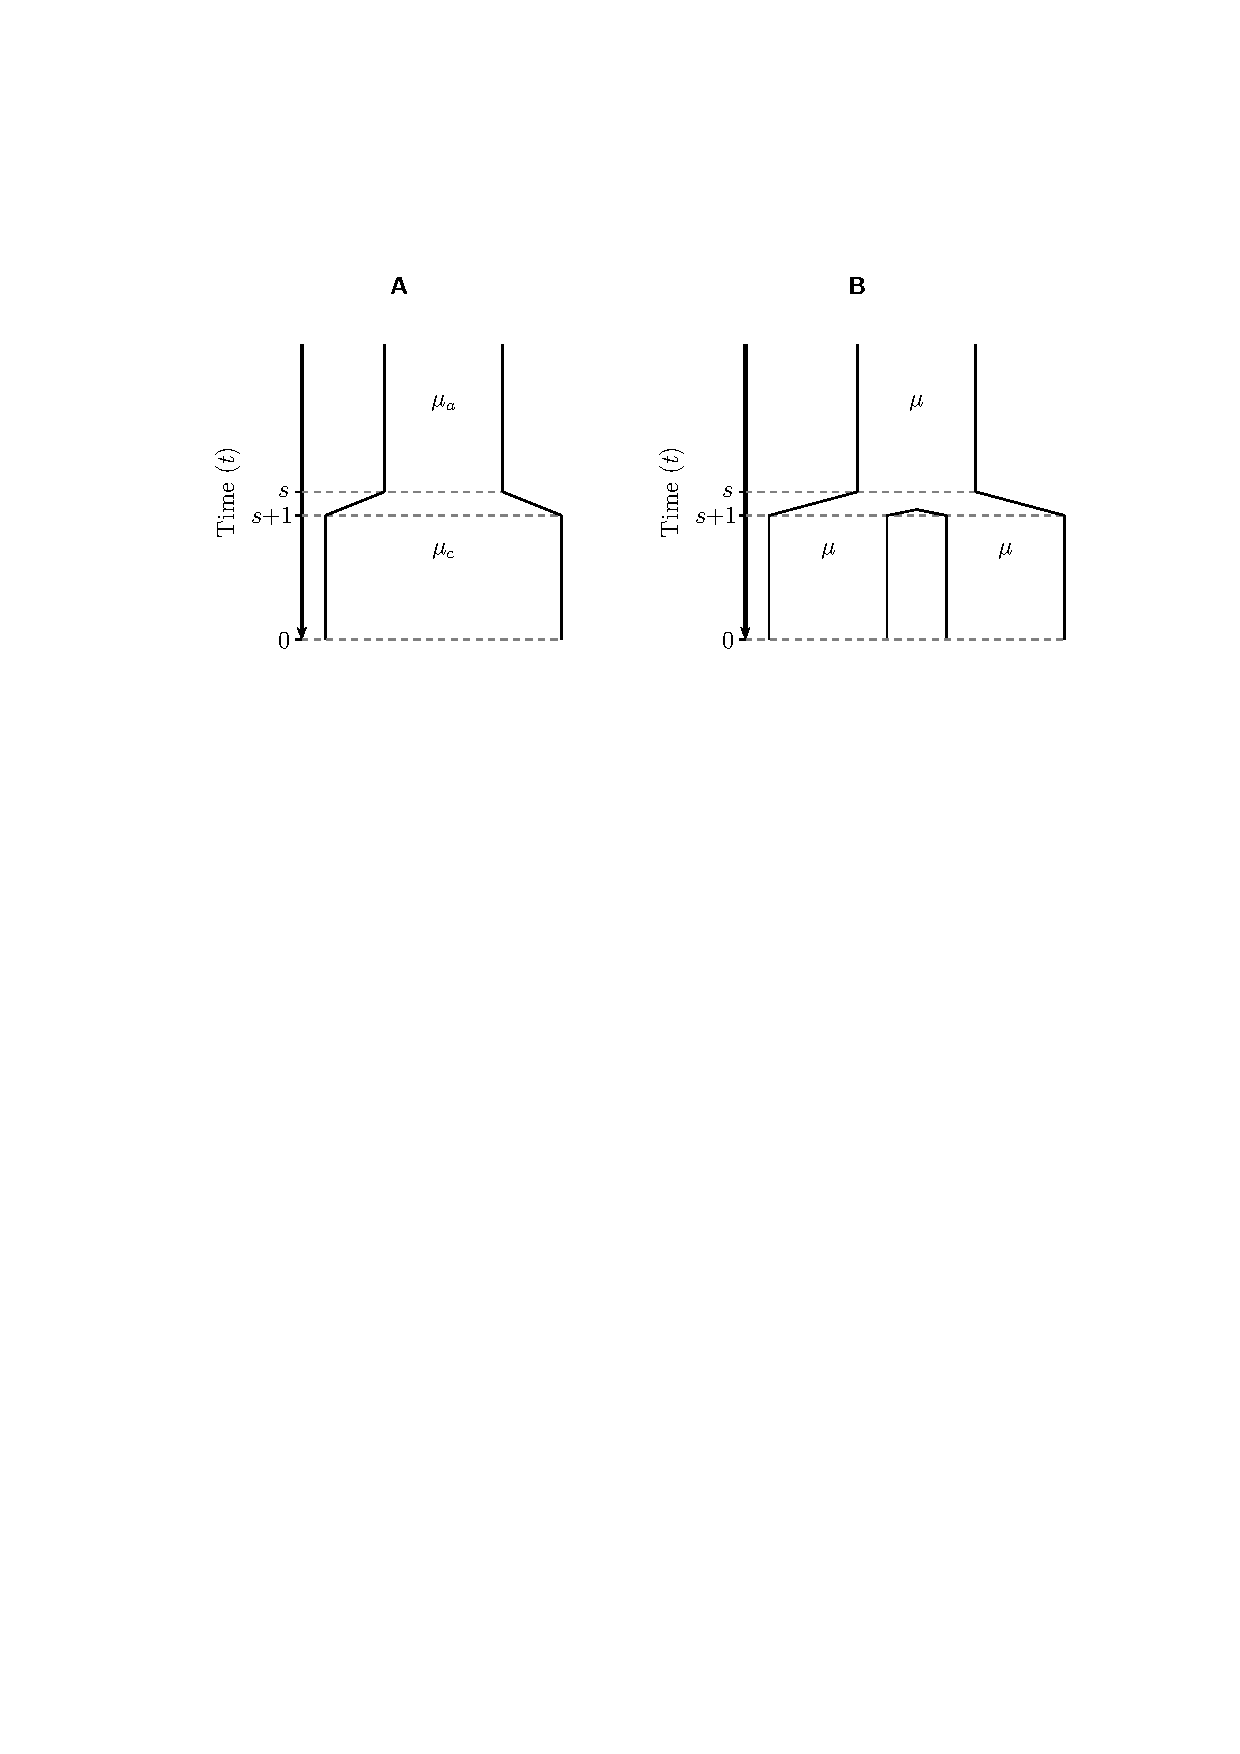
\includegraphics[width = 12cm]{diags.pdf}
\caption{Demographic scenarios. A) Population expansion. B) Population split.}\label{diag}
\end{figure}

\begin{figure}[ht]
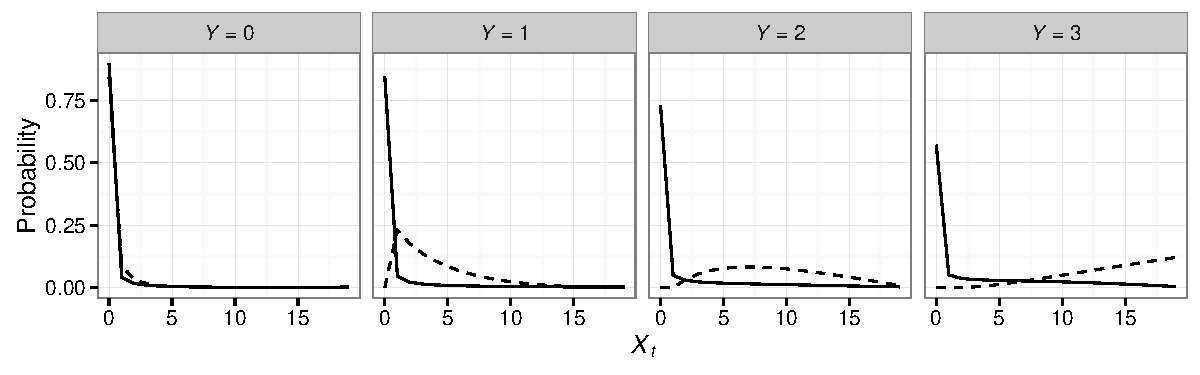
\includegraphics[width = 12cm]{cProb.pdf}
\caption{Conditional probabilities of allelic states in a site frequency spectrum of size $M=3$. The solid lines represent the conditional probabilities of an allelic state $\y$ at $t=s$, while the dashed lines represent the probabilities at $t=0$. The parameters were set to $\mu_a=0.05$, $\mu_c=0.1$, $s=-200$ and $N=20$.}\label{cProb}
\end{figure}

\begin{figure}[ht]
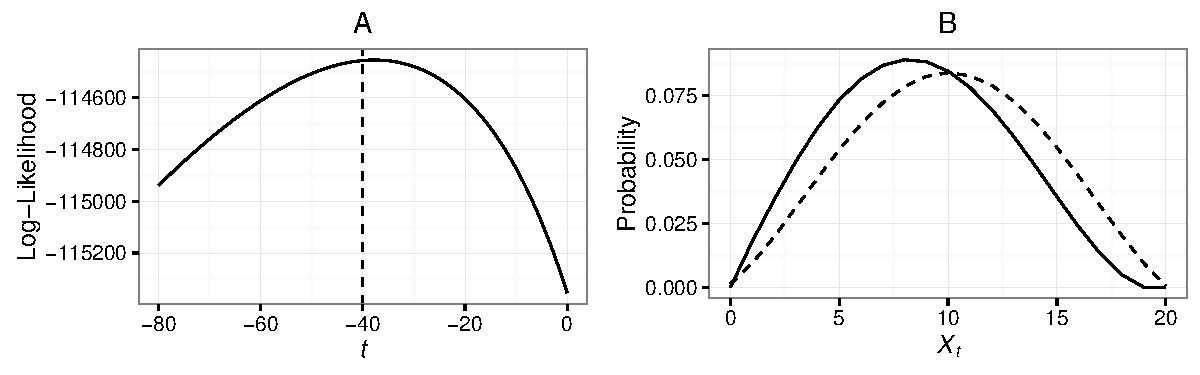
\includegraphics[width = 12cm]{twoPop_29_8_2016.pdf}
\caption{A) The log-likelihood of the split time $t$, given a jSFS (Table~\ref{jointSFSdiscr}). The dashed line indicates the true split time. B) The conditional probability for the allelic state with $y_1=1$ and $y_2=2$, at $t=s$ (solid line) and $t=0$ (dashed line).}\label{twoPopdiscr}
\end{figure}

\begin{figure}[ht]
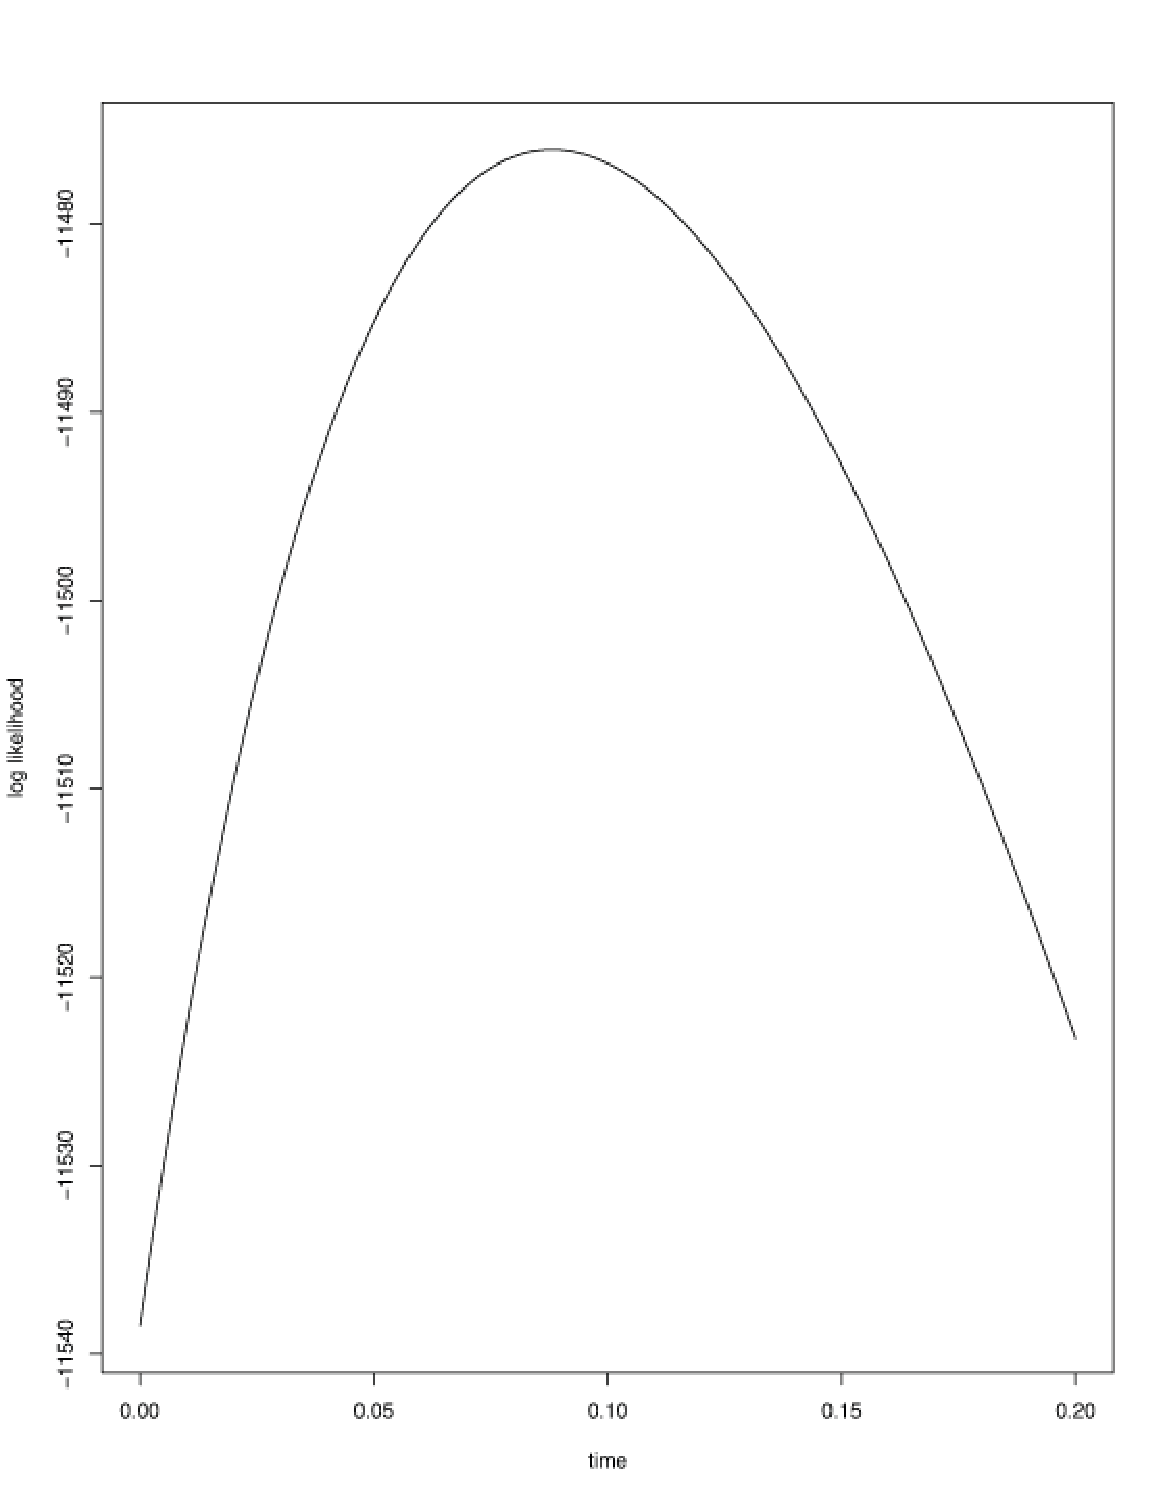
\includegraphics[width = 6cm]{forw_back_ll_cont.pdf}
\caption{The log-likelihood of the split time $f$, given a jSFS (Table~\ref{jointSFScont}). The dashed line indicates the true split time.}\label{twoPopcont}
\end{figure}

\clearpage

\section*{Tables}

\begin{table}[ht]
\centering
%\fontsize{5}{5}\selectfont
\caption{A jSFS simulated with a discrete Moran model with parameters $L=10^5$, $M_1=M_2=3$, $\alpha=2/3$, $\theta=0.1$, $s=-40$ and $N=20$.}
  \begin{tabular}{lllll}
  \toprule
    $\y$&$0$&$1$&$2$&$3$\\
    \midrule
    $0$  &$29037$ &$1315$ &$436$  &$185$\\ 
    $1$  &$1276$  &$688$  &$539$  &$432$\\  
    $2$  &$446$   &$529$  &$662$  &$1524$\\  
    $3$  &$202$   &$507$  &$1430$ &$60792$\\
    \bottomrule
  \end{tabular}\label{jointSFSdiscr}
\end{table}

\begin{table}[ht]
\centering
%\fontsize{5}{5}\selectfont
\caption{A jSFS simulated with a continuous diffusion model with parameters $L=10^5$, $M_1=M_2=3$, $\alpha=2/3$, $\theta=0.1$, and $s=-0.1$.}
  \begin{tabular}{lllll}
  \toprule
    $y$&$0$&$1$&$2$&$3$\\
    \midrule
    $0$  &$28877$ &$1447$ &$494$  &$231$\\
    $1$  &$1448$  &$570$  &$491$  &$557$\\
    $2$  &$497$   &$516$  &$543$  &$1491$\\
    $3$  &$253$   &$521$  &$1506$ &$60558$\\
    \bottomrule
  \end{tabular}\label{jointSFScont}
\end{table}

% \subsection{Appendix: Derivation of the continuous boundary mutation model from the discrete boundary mutation model}

% The forward discrete boundary mutation model may be written as
% \begin{equation}\label{eq:forw_discr_bound_mutation}
% \begin{split}
% &\Pr(\x{t+1}=i)-\Pr(\x{t}=i) = \\
% &\qquad \frac{\alpha\theta N}{N^2} \bigg[\Pr(\x{t}=i-1)\delta_{i-1,0} - \Pr(\x{t}=i)\delta_{i,0}\bigg]\\
% &\qquad+\frac{\beta\theta N}{N^2} \bigg[\Pr(\x{t}=i+1)\delta_{i+1,N} - \Pr(\x{t}=i)\delta_{i+1,N}\bigg]\\
% &\qquad+\frac1{N^2}\bigg[(i-1)(N-i+1)\Pr(\x{t}=i-1) \\
% &\qquad+ (i+1)(N-i-1)\Pr(\x{t}=i+1)-2i(N-i)\Pr(\x{t}=i)\bigg]\,,
% \end{split}
% \end{equation}
% where $\delta_{i,j}$ is one if $i=j$ and zero otherwise. 

% As with the derivation from the general model, we use the measure~(\ref{eq:measure}). For $\x{0}$, we have again (now without invoking fast drift towards the boundaries)
% \begin{equation}
% \begin{split}
% \frac{\Pr(\x{\tau}=0)-\Pr(\x{\tau}=0)}{\delta \tau} =
% &-\alpha\theta \frac{\Pr(\x{\tau}=0)}{\delta x}
% +\frac{\delta x (1-\delta x)\phi(x+\delta x,\tau)\delta x}{\delta x^2}\,.\\
% \end{split}
% \end{equation}
% From this the loss through drift, \ie\ eq.~\label{eq:forw_lossdrift} can be obtained. Considerations with respect to mutation are more complicated. Generally the mutation rate needs to be compensated b


% The first term represents loss from the boundary through mutation, the second gain through drift. Conversely, the rates of loss through drift towards the boundaries therefore are
% \begin{align}\label{eq:forw_lossdrift}
%   \begin{cases}
%     (1-\delta x)\phi(x=\delta x,\tau) &\text{at $x=\delta x$ and}\\
%     (1-\delta x)\phi(x=1-\delta x,\tau) &\text{at $x=1-\delta x$.}\\
% \end{cases}
% \end{align}
% $\Pr(\x{\tau}=0)$ quickly converges to $b_0(\tau)$ and $\Pr(\x{\tau}=1)$ to $b_1(\tau)$% and the change of the boundary terms is so slow that the left side of eq.~(\ref{eq:bound:dynamics_0}) can be set to zero
% . Therefore $b_0(\tau)$ is always available for mutation at the boundary $x=0$ and $b_1(\tau)$ at the boundary $x=1$ and the interior receives through mutation from the boundaries:
% \begin{equation}\label{eq:forw_gainmut}
% \begin{cases}
% \alpha\theta \frac{b_0(\tau)}{\delta x} &\text{at $x=\delta x$, and}\\
% \beta\theta\frac{b_1(\tau)}{\delta x} &\text{at $x=1-\delta x$.}\\
% \end{cases}
% \end{equation}
% At the boundaries, dynamics are slow compared to the region inside, in particular, 
% \begin{equation}\label{eq:forw_boundaries}
%     \frac{d}{d\tau}b_1(\tau)=-b_1(\tau)+\alpha\,.
% \end{equation}
% Within the interval $\delta x\leq x \leq 1-\delta x$, dynamics are governed by the pure drift diffusion equation
% \begin{equation}\label{eq:forw_drift}
%   \frac{\partial}{\partial \tau} \phi(x,\tau) =\frac{\partial^2}{\partial x^2}x(1-x)\,\phi(x,\tau)\,.  
% \end{equation}
% Equations (\ref{eq:forw_lossdrift})-(\ref{eq:forw_drift}) completely specify the forward dynamics of the boundary mutation-drift model.

% \subsection{Appendix: maybe useless}

% Note that the forward expansion (\ref{eq:forw_expansion_boundary}) can be rearranged as follows. The expansion of the stationary distribution \label{eq:forw_bounddrift} is
% \todo[inline]{Check signs!}
% \begin{equation}
%     H_0^{'}(x)=\pi(x, \alpha, \theta)= H_0(x)+\sum_{i=2}^\infty A_n H_n(x)
% \end{equation}
% and similarly
% \begin{equation}
%     H_1^{'}(x)=H_1(x)+ \sum_{i=2}^\infty B_n H_n(x)\,.
% \end{equation}
% Furthermore, we set 
% \begin{equation}
% \begin{split}
%     a_0^{'}&=a_0-\sum_{i=2}^\infty a_n\frac{(-1)^n+1}{i}\,,\\
%     a_1^{'}&=a_1-\sum_{i=2}^\infty a_n\frac{(-1)^n\alpha -\beta}{i}\,.
% \end{split}
% \end{equation}
% Then the time-dependent functions for $n\geq 2$ become
% \begin{equation}
% \begin{split}
%     T_0^{'}(\tau)&=a_0^{'}1+\sum_{i=2}^\infty e^{-n(n-1)\tau}\,,\\
%     T_1^{'}(\tau)&=a_1^{'}e^{\theta \tau} +\sum_{i=2}^\infty a_1 B_n (e^{-\theta t}-e^{-n(n-1) \tau})\,,\\
%     T_n^{'}(\tau)&=(a_n-a_0 A_n)e^{-n(n-1)\tau}\,.
% \end{split}
% \end{equation}
% With these redefinitions the forward expansion becomes
% \begin{equation}\label{eq:forw_expansion_boundary}
% \begin{split}
%     &\phi(x,t)= T_0(\tau)\,H_0^{'}(x)+T_1(\tau)\,H_1^{'}(x)+\sum_{n=2}^\infty e^{-n(n-1)\tau}\,H_n(x)\,.
% \end{split}
% \end{equation}
% Truncated at some $n=n_{max}$ the latter version of the forward expansion is much smoother than the former. Furthermore,  $H_0^{'}(x)$ and $H_1^{'}(x)$ may be replaced by beta functions, as well as the boundary terms of the $H_n(x)$, such that the discontinuities at the boundaries are not necessary. The latter version thus seems preferable, if only the forward diffusion is needed, but only the former is orthogonal with the backward functions we develop below.


% \subsection{Example: irreversible boundary mutation model}
% \label{section:irreversible_diffusion}

% Similar considerations to above also apply to the model in section~(\ref{section:irreversible}) with irreversible mutation, \ie\ where the ancestral and derived states are contrasted. Note that \citet{Evan07} arrive at the same irreversible diffusion model from a Wright-Fisher model and provide recursive equations of moments instead of orthogonal polynomials to calculate the expected SFS under non-equilibrium conditions. \citet{Zivk11} extend their analysis to provide the solution backward in time.  If $N\to\infty$, $\theta/(1-\theta\sum_{i=1}^{N-1}1/i)$ goes to infinity, such that the model collapses. Hence, we assume that mutations constantly supply probability mass from the boundaries to $x=1/N$ at rate $N\theta$ (after scaling time). The forward diffusion equation then becomes
% \begin{equation}\label{eq:forw_onebounddrift}
% \begin{split}
% \frac{\partial}{\partial \tau} \phi(x,\tau)&=
%     \lim_{N\to\infty} N\theta \delta(x-\tfrac1N)b+\frac{\partial^2}{\partial x^2}x(1-x)\,\phi(x,\tau)\,.
% \end{split}
% \end{equation}
% The term $b$ corresponds to the probability $\int_0^1\phi(x,\tau=0)\,dx$, which is unity if the initial distribution integrates to one. The equilibrium distribution is 
% \begin{equation}
% \begin{split}
%     \pi(x\given\theta)&=\left(1-\lim_{N\to\infty}\theta \int_{\tfrac1N}^{\tfrac{N-1}N} \frac1x\,dx\right)\delta(x)+\theta\frac{1}{x(1-x)}\,.
% \end{split}
% \end{equation}
% The augmented eigenfunctions are for $n\geq 2$
% \begin{equation}\label{eq:forw_onebound_eigen}
%     H_n(x)=\tfrac{(-1)^n+1}{n}\delta(x)+U_n(x)\,,
% \end{equation}
% while the zeroth and first eigenfunctions collapse to $\delta(x)$.

% Substituting $\sum_nT_n(\tau) H_n(x)$ into the forward differential equation (\ref{eq:forw_onebounddrift}) results in the inhomogeneous linear differential equation describing the time-dependent part of the solution
%\begin{equation}\label{eq:inhomogeneous}
%    \frac{d}{d\tau}T_n(\tau)=-\lambda T_n(\tau)-\theta (2n-1)n(-1)^n\,.
%\end{equation}


%Consider a sample of size $M=2$, where $y \in (0,1,2)$ and assume stationarity. The likelihoods are $\Pr(y\given M=2)=\binom{2}{y}x^{y}(1-x)^{M-y}$ such that the joint probabilities under stationarity are for $y=1$: $\Pr(x,y=1\given M=2)=\theta 2(1-x)$ and for $y=2$: $\Pr(x,y=1\given M=2)=\theta x$. They can easily be expanded into polynomials $H_n(x)$ up to order $n=3$. For both, the boundary term at $\tau=0$ must be zero, such that $b=\theta$ and $b=\theta/2$, for $y=1$ and $y=2$, respectively. For $y=0$, we have inside the polymorphic region the expansion $\theta (1-x)^2/x=\sum_{n=0}^\infty x^{n+2}$ and at the boundary $b=1-3\theta/2$. Substituting these initial values into the inhomogeneous differential equations (\ref{eq:inhomogeneous}) results in the expansion for all $\tau>0$.

%Consider again a sample of size $M=2$, where $y \in (0,1,2)$. With $y=1$, initially $T_2(\tau=0)=2$, while all $T_n(\tau=0)$ with $n>2$ are zero. Since the boundary term is initially zero, $b=\theta$ in the backward diffusion equation (\ref{eq:backw_onebounddrift}). Another way to derive the boundary term is to note that it is equal to $\Pr(y=1\given \theta)=\theta$. Substituting these initial values into the inhomogeneous differential equations (\ref{eq:inhomogeneous}) results in the expansion for all $\tau$. The backward expansion converges to a constant distribution $\theta$ within the interval including zero but excluding one with $\tau\to\infty$.

%With $y=0$, we initially expand $x/(1-x)$ into a polynomial $\sum_{n=0}^\infty x^{n+1}$ and determine the $T_n(x)$, while the boundary term is equal to $\Pr(y=0\given \theta)=\theta/2$. With $y=2$, the expansion is similar to that with $y=0$, but reflected around $x=1/2$, while the boundary term is equal to $\Pr(y=2\given \theta)=1-3\theta/2$.

\end{document}

%%% Local Variables:
%%% mode: latex
%%% TeX-master: t
%%% End:
